\documentclass{book}
\usepackage[letterpaper, total={6.5in,9in}]{geometry}
\usepackage{amsmath}
\usepackage{physics}
\usepackage{hyperref}
\usepackage{xcolor}
\usepackage{graphicx}
\usepackage{float}
\graphicspath{/Users/collinsinclair/Documents/School/2021/sp21/ASTR 3830/finalExam/images}
\hypersetup{
    colorlinks,
    linkcolor=black,
    citecolor=blue,
    urlcolor=blue
}
\title{ASTR 3830: Astrophysics 2 – Galactic and Extragalactic \\
Final Exam Review Guide}
\author{The Students of ASTR 3830}
\begin{document}
\maketitle
\tableofcontents
\chapter{Exam 1 Content}
\section{The Milky Way (C\&O Chapter 24)}
\subsection{Determining Morphology of the Milky Way}
\subsubsection{Magnitudes}
\begin{itemize}
    \item M: Absolute magnitude, magnitude as seen at 10 pc?
    \item m: Apparent magnitude, magnitude as seen at observer’s distance
    \item Small magnitude = brighter
    \item Big mag = dimmer
    \item It’s backwards
    \item Pro tip: when looking at a plot, take your time to orient yourself (which is left, which is right, up, down, brighter, dimmer, more massive, less massive, etc) because astronomers are out of their minds and don’t make graphs like normal people.
\end{itemize}
The Milky Way is a SBb-SBc bar spiral.
\subsection{Filter Systems}
\begin{itemize}
    \item F(\#\#\#) - filter (centered at) note to watch out for inferred numbers
          \begin{itemize}
              \item Example: U365
          \end{itemize}
    \item Standard UBV System (Johnson system):
          \begin{itemize}
              \item U - ultraviolet centered at 365 nm
              \item B - blue centered at 440 nm
              \item V - visual centered at 550 nm
          \end{itemize}
    \item Extension: UBVRI
          \begin{itemize}
              \item R - red
              \item I - Infrared
          \end{itemize}
\end{itemize}
\begin{center}
    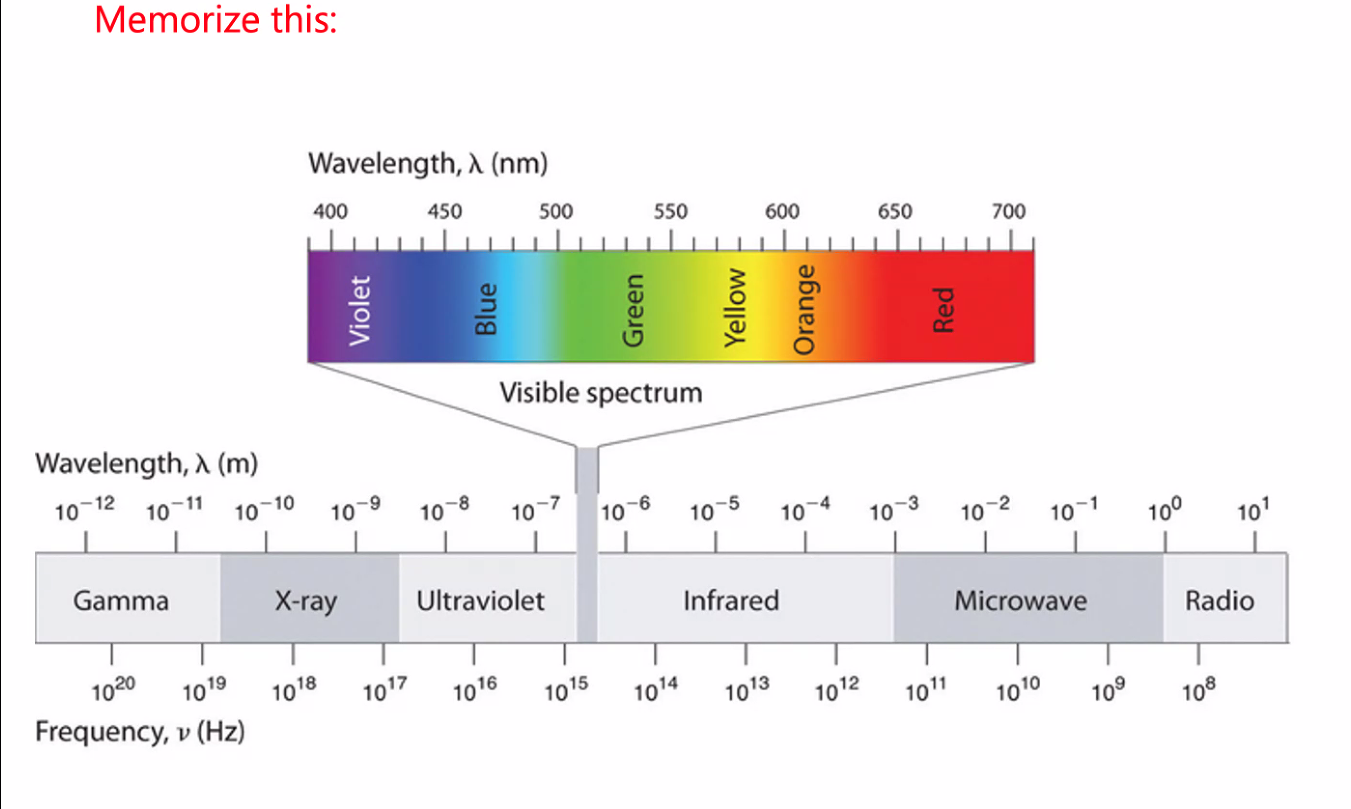
\includegraphics[height = 0.45\textwidth]{images/emspectrum.png}
\end{center}
\subsection{Differential Star Count}
\begin{itemize}
    \item Counts the number of stars with an absolute magnitude between $M$ and $M = dM$ that are found within a solid angle $\Omega$ and have apparent magnitudes in the range between $m$ and $m  + dm$:
          \begin{equation*}
              A_M (M, S, \Omega, m)\ dM\ dm \equiv \frac{d\bar{N}_M (M, S, \Omega, m)}{dm}\ dM\ dm \tag{C\&O 24.4}
          \end{equation*}
    \item In special case where we assume no interstellar extinction ($A=0$) and infinite universe of uniform stellar density (i.e. $n_M(M, S, \Omega, r) = n_M(M, S) = $ constant),
          \begin{align*}
              A_M (M, S, \Omega, m) & = \frac{d\bar{N}_m (M, S, \Omega, m)}{dm}                       \\
                                    & = \frac{\ln 10}{5} \Omega n_m (M, S) 10^{3(m - M +5)/5}         \\
                                    & = \frac{3 \ln 10}{5} \bar{N}_M(M, S, \Omega, r) \tag{C\&O 24.5}
          \end{align*}
\end{itemize}
\subsection{Integrated Star Count}
\begin{itemize}
    \item Counts the total number of stars with absolute magnitudes in the range $M$ to $M + dM$ that appear brighter than the limiting magnitude, $m$ (replaces the limiting distance $r$ - see C\&O 24.1):
          \begin{equation*}
              n(S, \Omega, r) = \int_{- \infty}^\infty n_M (M, S, \Omega, r)\ dM \tag{C\&O 24.2}
          \end{equation*}
          where $n_M (M, S, \Omega, r)\ dM$ is the number density of stars with attribute $S$ that lie within a solid angle $\Omega$ in a specific direction.
    \item In the special case where we assume no interstellar extinction ($A=0$) and infinite universe of uniform stellar density (i.e. $n_M(M, S, \Omega, r) = n_M(M, S) = $ constant),
          \begin{align*}
              \bar{N}_M (M, S, \Omega, m) & = \frac{\Omega}{3} n_M (M, S) 10^{3 (m - M + 5)/5}                        \\
                                          & = \frac{\Omega}{3} n_M (M, S) \exp\left( \ln 10^{3 (m - M + 5)/5} \right) \\
                                          & = \frac{\Omega}{3} n_M (M, S) e^{[3 (m - M + 5)/5]\ln 10}
          \end{align*}
\end{itemize}
\subsection{Obscuration}
\begin{itemize}
    \item Use distance to solve for extinction $A_\lambda$:
          \begin{equation*}
              d = 10^{(m_\lambda - M_\lambda - A_\lambda + 5)/5} \implies A_\lambda = m_\lambda - M_\lambda + 5 - 5 \log_{10} d \tag{C\&O 24.1}
          \end{equation*}
    \item Observe using infrared (longer wavelengths) to penetrate dust
\end{itemize}
\subsection{Milky Way Components}
\begin{center}
    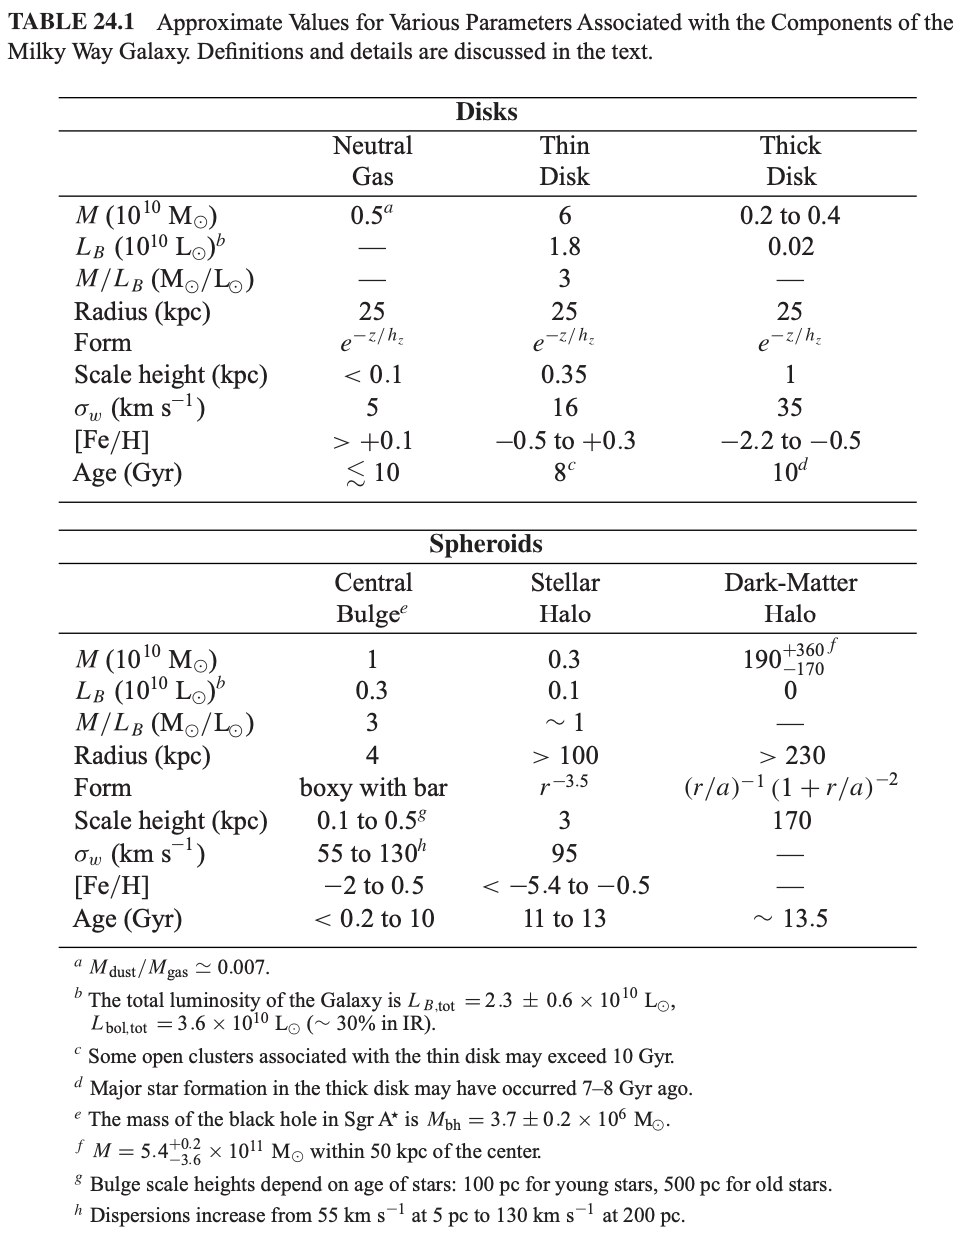
\includegraphics[height=\textwidth]{images/co_table24_1.png}
\end{center}
\subsection{Milky Way Kinematics}
\begin{itemize}
    \item Does not follow Keplerian model, Flat velocity curve
    \item Density wave theory: explains the winding problem and how stars move in and out of the spiral arms, the spiral arms originate from quasi-static density waves -- traffic build up example. Each star has its tilted stellar orbits
    \item Perigalacticon/Apogalacticon calculation

\end{itemize}
\subsection{Galaxy Rotation Curves}
\begin{itemize}
    \item Doesn’t follow Keplerian model
    \item Flattens out at higher radii, follows Keplerian at smaller radii
    \item Rotation curve is determined by the mass enclosed (light matter and dark matter)
    \item Inner region (up to $\sim 5\ kpc$), density of stars goes as $\sim 1/r$, velocity goes as $\sim \sqrt{2}$
    \item Outer region, need density go as $\sim 1/r^2$ to create flat rotation curve, velocity goes as $\sim 1 / \sqrt{r}$
          \begin{itemize}
              \item  $M_r$ becomes constant
          \end{itemize}
\end{itemize}
\subsection{Evidence for Dark Matter}
\begin{itemize}
    \item It is not gas. Hot gas would have emission lines, cold gas would have absorption lines
    \item It is not asteroids, rocks or dust: there isn’t enough
    \item Flat rotation curves
    \item Mass-to-light ratio: the ratio between the measured luminosity and the estimated mass. It does not account for the rotation of the stars.
    \item Gravitational lensing
\end{itemize}
\subsection{MACHOs, WIMPs}
\begin{itemize}
    \item MACHO: massive compact halo objects: brown dwarfs, white dwarfs, neutron stars, black holes, etc.
    \item WIMPs: weakly interacting massive particles (neutrinos)
    \item Both possible explanations for dark matter
    \item Does not explain all the mass expected
\end{itemize}
\subsection{NFW Profile}
\begin{itemize}
    \item NFW density profile
          \begin{equation*}
              \rho_{NFW} (r) = \frac{\rho_0}{(r/a)(1+r/a)^2} \tag{C\&O 24.52}
          \end{equation*}
    \item Averages out to be $1/r^2$ over much of the halo to explain that velocity = constant on the rotation curves
    \item Shallow near the center $(\sim 1/r$) near the center
    \item Steeper ($\sim 1/r^3$) near the edge of the halo
    \item Total mass contained within NFW profile is still not bound (like problem 4 in homework)
    \item For galaxies, $a \sim 10-30\ kpc$ (scale radius)
\end{itemize}
\subsection{Galactic Center Observations}
\begin{itemize}
    \item $1\ m$ wavelength $\implies$ radio
    \item Adaptive optics: Keck Telescope using adaptive optics (AO) to observe $Sgr\ A^*$
\end{itemize}
\subsection{Evidence for a SMBH in the Galactic Center}
\begin{itemize}
    \item Rotation of S2 and other stars around the center of the galaxy. (Seen through the microwave)
    \item No other explanation besides a SMBH.
    \item X-ray emission.
    \item Used orbits of stars to calculate mass of center $= 3.7 \pm 0.2 \times 10^6\ M_\odot$
\end{itemize}
\subsection{Virial Theorem}
\begin{equation*}
    \langle E \rangle = \langle K \rangle + \langle U \rangle
\end{equation*}
\begin{itemize}
    \item See Lecture 3, Section 2.4 of C\&O
    \item $-2 \langle K \rangle = \langle U \rangle$
          \begin{itemize}
              \item Note: This form applies to special case where galaxy is in equilibrium and gravitationally bound
          \end{itemize}
\end{itemize}
\subsection{Sgr A$^*$ Luminosity Function}
\begin{itemize}
    \item Luminosity comes from accretion
    \item Using the virial theorem: $\langle E \rangle = \frac{1}{2} \langle U \rangle$
    \item Luminosity is $dE/dt$
\end{itemize}
\section{The Nature of Galaxies (C\&O Chapter 25)}
\subsection{The Great Debate Over Spiral Nebulae}
\begin{itemize}
    \item Side 1) The mysterious “spiral nebulae” are nebulae within our own galaxy
    \item Side 2) They are outside our galaxy - ``island universes''
    \item Shapley: supported idea of nebulae being in our Galaxy - argued using apparent magnitudes of novae - argued that if the disk of Andromeda were as large as the Milky Way, then its angular size in the sky would imply a distance to the nebula so large that luminosities of novae would be greater than those found in Milky Way. Also argued the points of Maanen: proper-motion measurements of M101 suggest angular rotation of $0.02"\ yr^{-1}$, if diameter similar to Milky Way then why rotational speed not larger?
    \item Curtis: supported the idea of spiral nebulae Being outside our Galaxy - argued that the novae observed must be at least 150kpc away in order to have intrinsic brightnesses comparable to those in the Milky Way. Also argued that the large radial velocities measured for spiral nebulae indicated they could not remain gravitationally bound within a Kapteyn-model Milky Way. (Lecture 1)
\end{itemize}
Curtis was proven correct when Hubble detected Cepheid variable stars in M31. Using apparent magnitudes to determine absolute magnitudes, and then using the period-luminosity relation:
\begin{equation*}
    M_{\langle V \rangle} = -2.81 \log_{10}(P_d) - 1.43 \tag{C\&O 14.1}
\end{equation*}
where $M_{\langle V \rangle}$ is the average absolute $V$ magnitude and $P_d$ is the pulsation period in units of days.

Hubble was able to approximately calculate the distance to Andromeda to be outside the Milky Way Galaxy.
\subsection{Galaxy Morphologies, Hubble Classification Scheme}
\begin{center}
    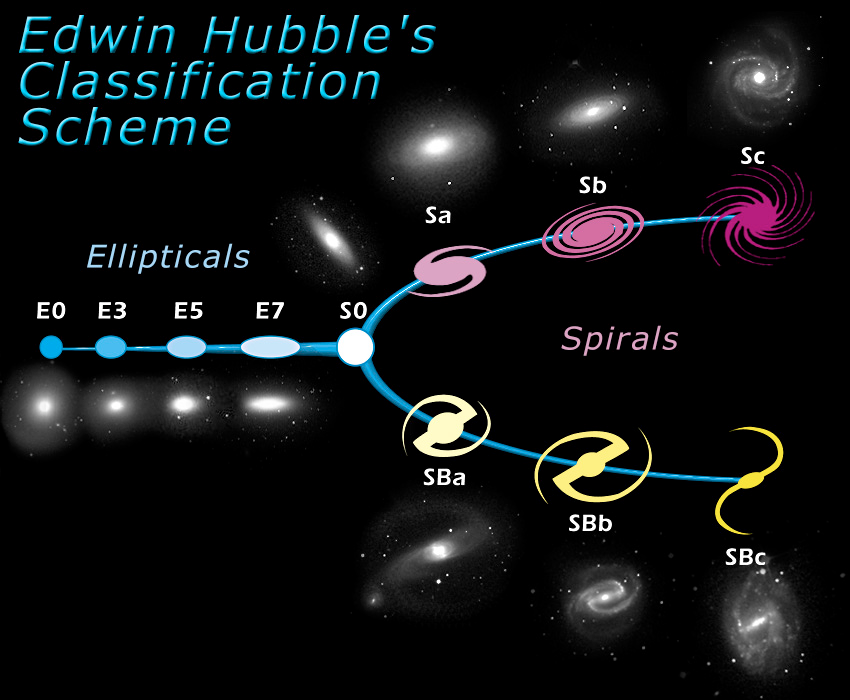
\includegraphics[height = 0.4 \textwidth]{images/hubble_class.png}
\end{center}
\begin{itemize}
    \item 3 types: ellipticals, spirals, irregulars
    \item E0 $\to$ E7: greater ellipticity
    \item S0: disk, bulge, no arms
    \item Sa $\to$ Sc: lower bulge-to-disk size and luminosity ratios, spiral arms less tightly wound
    \item NOT an evolutionary sequence
    \item Observed ellipticity: $\epsilon = 1 - \beta / \alpha$
\end{itemize}
\begin{center}
    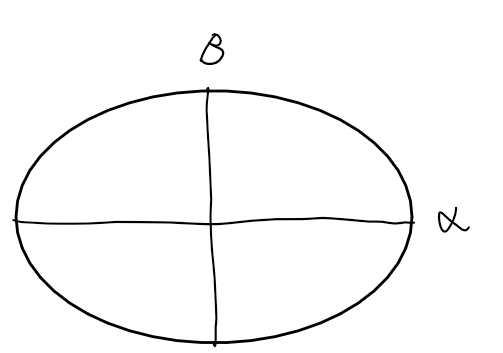
\includegraphics[height = 0.4 \textwidth]{images/ellipse.png}
\end{center}
\subsection{Galaxy Surface Brightness, Sérsic Profile}
\begin{itemize}
    \item A galaxy's surface brightness $\mu$ is the amount of flux from the galaxy per square arcsecond on the sky
    \item Calculate luminosity, then total flux from all stars
    \item Surface brightness is unrelated to distance
    \item Observer units: $\mu$ units: mag arcsec$^{-2}$
    \item Theorist units: $I$ units: $L_\odot\ pc^{-2}$
    \item K-correction: de-redshifted
    \item de Vaucouleurs Profile: surface brightness $I \sim r^{1/4}$ for spiral galaxy bulges and elliptical galaxies:
          \begin{equation*}
              \log_{10} \left[ \frac{I(r)}{I_e} \right] = -3.3307 \left[ \left( \frac{r}{r_e} \right)^{1/4} - 1 \right] \tag{C\&O 24.13}
          \end{equation*}
          where $I$ is the surface brightness measured in units of $L_\odot\ pc^{-2}$, $r_e$ is a reference radius (called the effective radius), and $I_e$ is the surface brightness at $r_e$. $r_e$ is defined to be that radius within which one-half of the bulge's light is emitted.
          \begin{itemize}
              \item \textbf{Note}: the equation above uses $I$ as the surface brightness which is consistent with C\&O, but in class we have used $\mu$ as the surface brightness.
          \end{itemize}
\end{itemize}
\subsection{How to Measure Rotation in Other Galaxies}
\begin{itemize}
    \item Neutral H in the interstellar medium
    \item The spin flip transition of HI emits photons of wavelength 21 cm
\end{itemize}
\begin{center}
    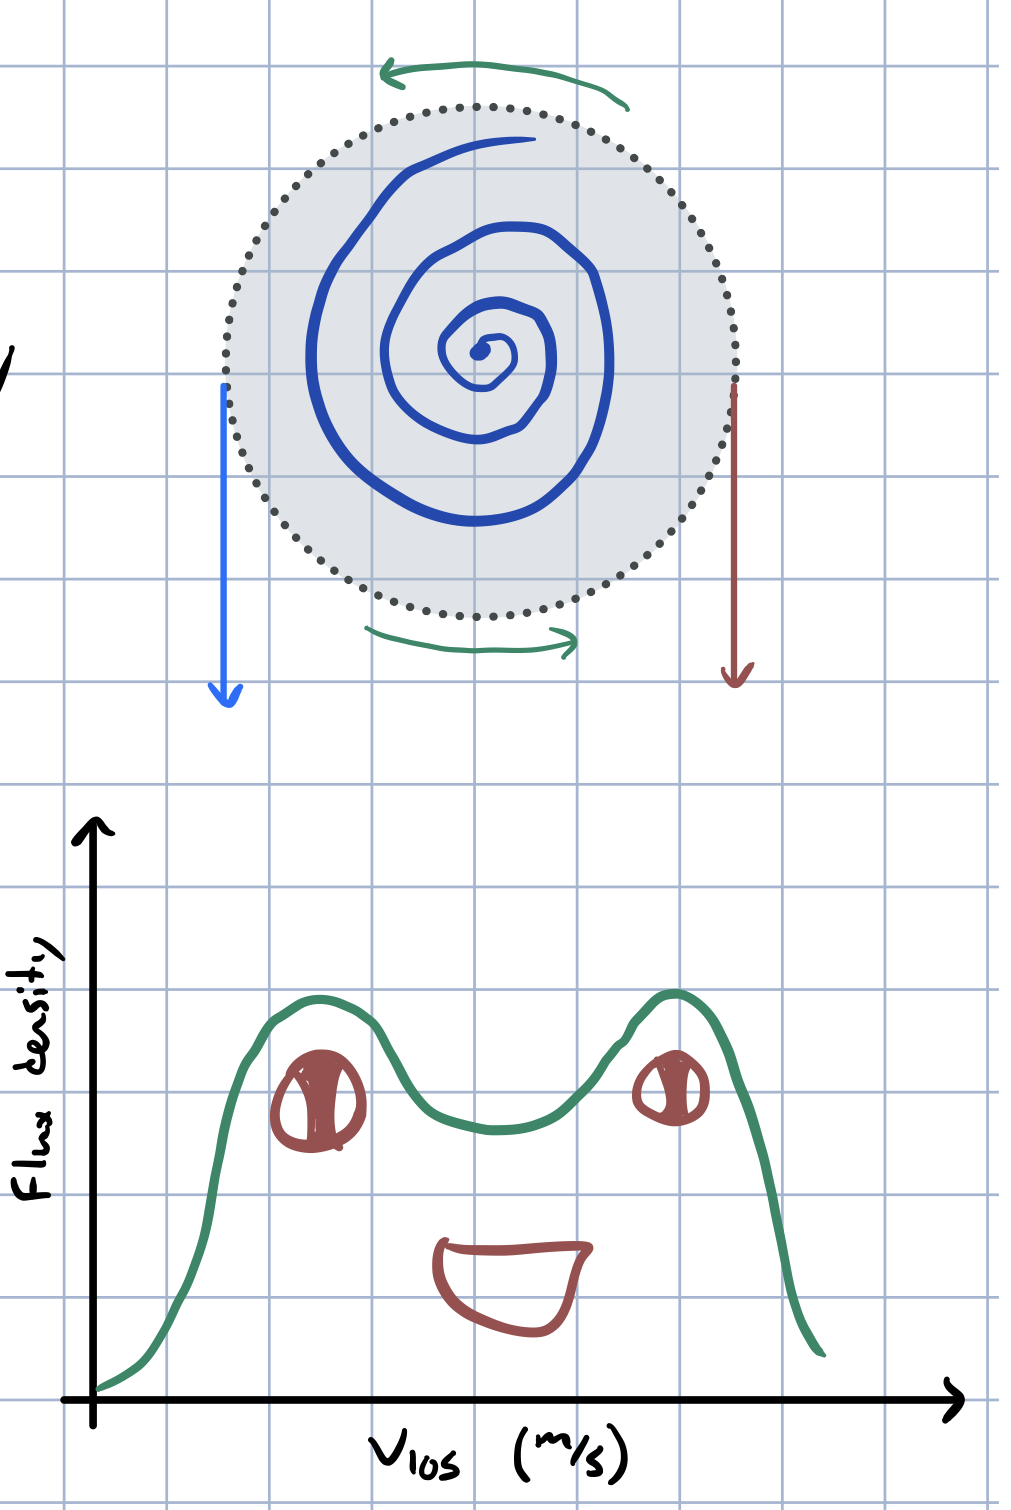
\includegraphics[height = 0.5 \textwidth]{images/rotation.png}
\end{center}
(Art courtesy of James l'Artiste.) Find $v_{max}$ with right peak - middle or left peak + middle
\subsection{Tully-Fisher Relation}
\begin{itemize}
    \item Tully and Fisher studied 21-cm emission lines in spiral galaxies and found that the absolute magnitude is related to the rotation
    \item $v_{max}$ is easiest to find, so measure $v_{max}$, use Tully-Fisher to get $M$ (absolute magnitude), and then distance - you also need $m$ (apparent magnitude)
\end{itemize}
\begin{center}
    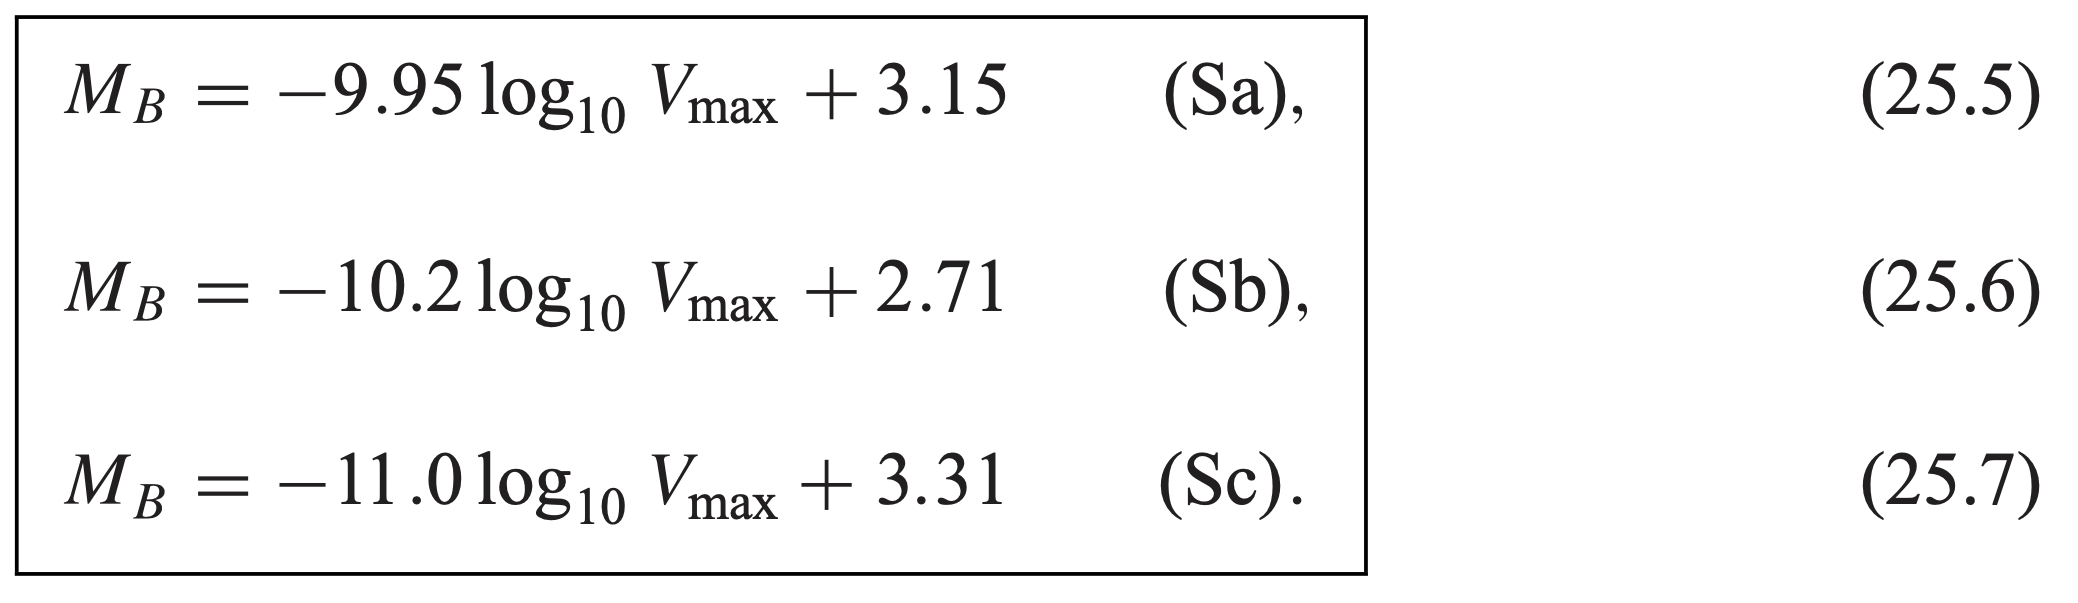
\includegraphics[width = \textwidth]{images/tullyfisher.png}
\end{center}
\subsection{Types of Spiral Arms}
\begin{itemize}
    \item Grand-design spiral: 2 large arms - 10\% of the spiral galaxy
    \item Multiple-arm: $>2$ large arms - 60\% of the spiral galaxy
    \item Flocculent spiral: Not well defined arms - 30\%
\end{itemize}
\subsection{Winding Problem, Density Wave Theory}
\begin{itemize}
    \item Traffic jam produced by slow moving truck (density wave) while cars (stars) slow down while moving around the truck.
    \item If we assume that all the stars in the galaxy stay together as they orbit, the spiral arms would wind up until we eventually have no spiral arms.
    \item This assumption is wrong, instead the stars constantly speed up or slow down as they enter and exit the spiral arms.
\end{itemize}
\begin{center}
    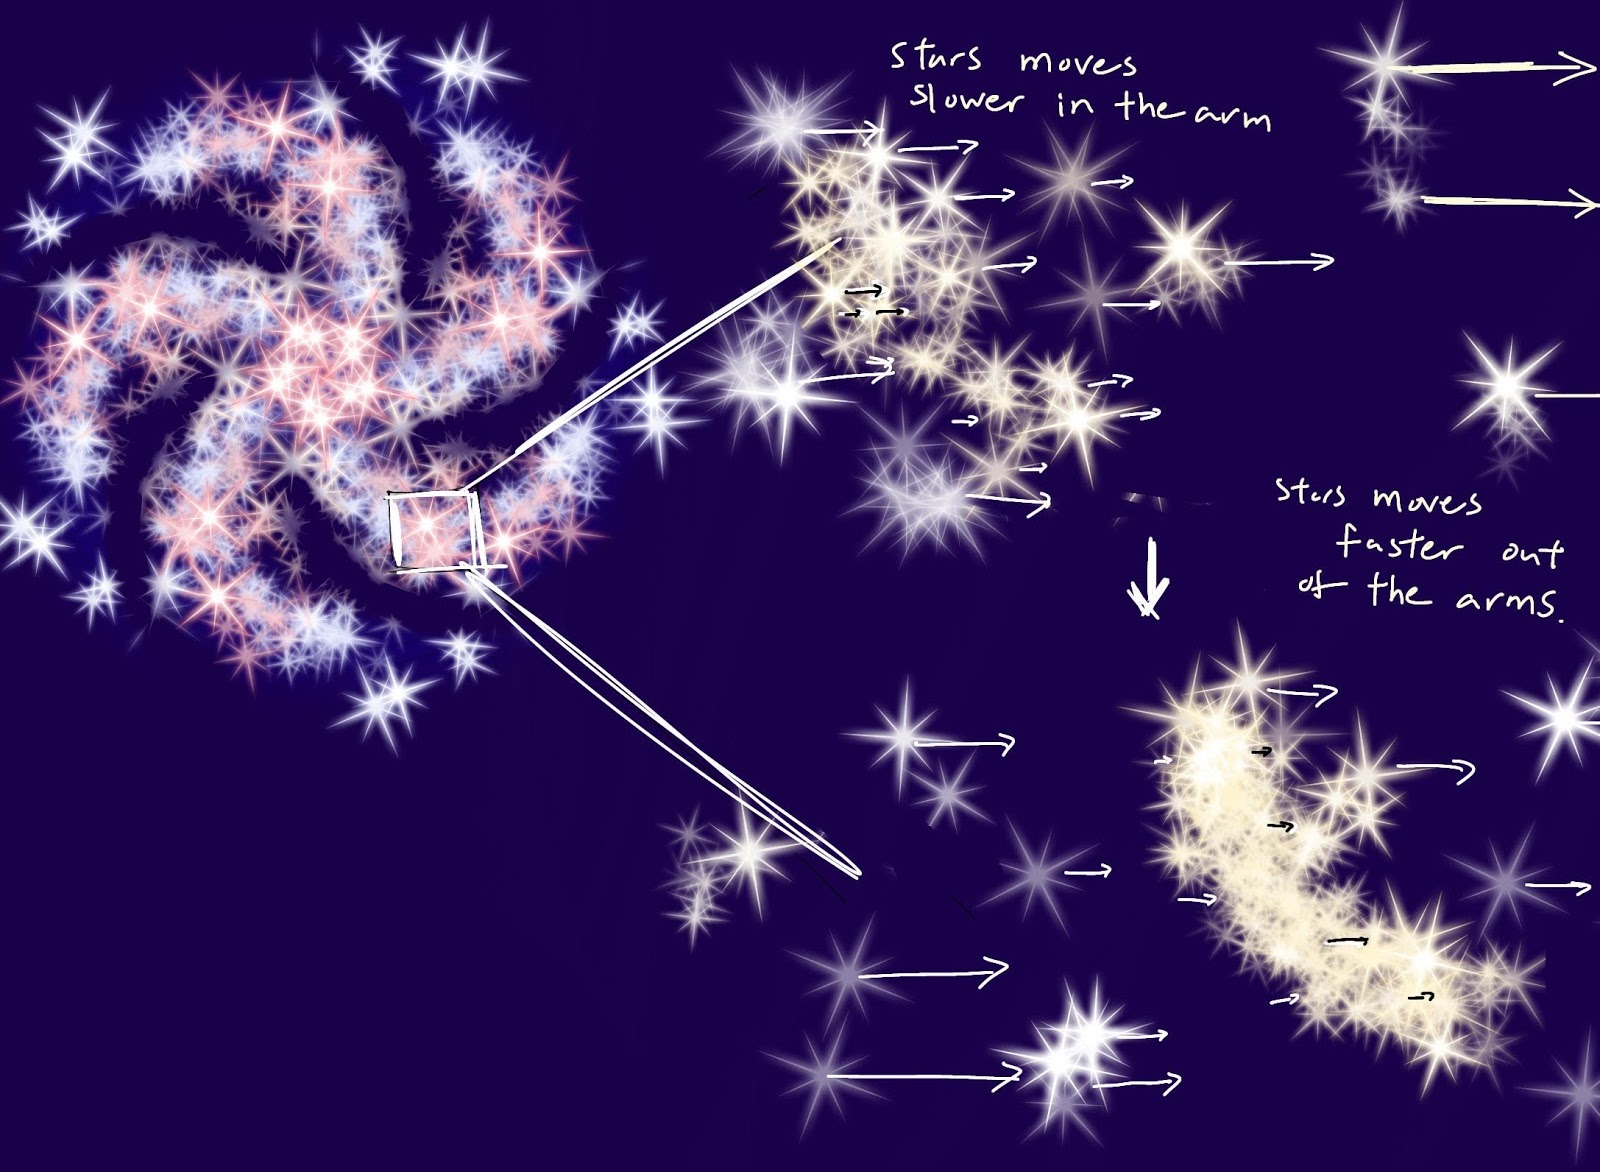
\includegraphics[width =0.7\textwidth]{images/winding.jpg}
\end{center}
\chapter{Exam 2 Content}
\section{The Nature of Galaxies}
\subsection{Spiral Galaxies versus Elliptical Galaxies: Major Differences}
\subsubsection{Spiral Galaxies}
\begin{itemize}
    \item Late-type in Hubble classification scheme
    \item Blue (which means less star formation!)
    \item Generally less luminous than ellipticals
    \item More abundant in the field
    \item Mass: $10^9$ to $10^{12} M_\odot$ (less massive on average)
\end{itemize}
\subsubsection{Elliptical Galaxies}
\begin{itemize}
    \item Early-type in Hubble classification scheme
    \item ``Red and dead'' (not forming new stars)
    \item Generally more luminous (brighter)
    \item More abundant in clusters
    \item Mass: $10^9$ to $10^{14} M_\odot$ (more massive on average)
\end{itemize}
\subsubsection{Bonus: Irrigular Galaxies!}
\begin{itemize}
    \item Sort of in between
    \item Usually the result of mergers
\end{itemize}
\subsection{Stellar Velocity Dispersion}
\begin{itemize}
    \item ``Statistical dispersion of stellar velocities around the man stellar velocity in a galaxy''
    \item Derived from the Virial Theorem to derive mass: $-2\langle K \rangle - \langle U \rangle$
          \begin{itemize}
              \item Assuming spherical distribution, $\langle v_r^2 \rangle = \sigma_r^2$ where $\sigma_r$ is the ``radial velocity dispersion''
          \end{itemize}
    \item Side note: \textbf{virial mass} $M \approx 5 R \sigma_r^2 / G$ can be used to calculate the total mass of an elliptical galaxy or the bulge of a spiral galaxy but not the whole spiral galaxy
    \item Measure stellar absorption lines, add them all up to make a galaxy spectrum and measure the velocity dispersion to get the total mass of a galaxy. The wider the absorption line, the more massive the galaxy.
\end{itemize}
\subsection{Faber-Jackson Relation}
\begin{itemize}
    \item Correlation between central velocity dispersion and luminosity
    \item Derived from the virial theorem
    \item For elliptical galaxies and spiral bulges (note: Tully-Fisher was for spiral galaxies)
    \item Brighter galaxies have larger velocity dispersions
    \item $L \propto \sigma^4 \propto L_\odot 10^{M_\odot/2.5}10^{-M/2.5}$ where $\sigma$ is the velocity dispersion and $L$ is the luminosity
    \item $\log (\sigma_r) \propto - M$
\end{itemize}
\subsection{The Fundamental Plane}
\begin{itemize}
    \item $\sigma$, luminosity, and size are the fundamental parameters of an elliptical galaxy or spherical bulge
    \item We often see 2D projections of the fundamental plane (i.e. Faber-Jackson relation)
\end{itemize}
\subsection{Galaxy Luminosity Function}
\begin{itemize}
    \item Relative number of galaxies at each luminosity
    \item Number density of galaxies in a particular sample that have luminosities between $L$ and $L + dL$: $$\Phi (L)\ dL = \frac{\sigma^*}{L^*} \left( \frac{L}{L^*}\right)^\alpha e^{-L/L^*}\ dL$$
    \item When $L \ll L^*$, $L \to 0$
    \item In magnitudes: $$\Phi(M) dM \approx 10^{0.4 (\alpha + 1) M}\exp\left( -10^{0.4(m^* - M)} \right)\ dM$$
    \item The ``knee'' is the turnover point where $\alpha = 1$
    \item To measure the luminosity function:
          \begin{enumerate}
              \item Measure the apparent magnitudes for all galaxies in the sample
              \item Convert to absolute magnitudes
              \item Calculate K-correction
              \item Count the number of galaxies in each K-corrected absolute magnitude bin, then divide te number of galaxies by the volume surveyed.
          \end{enumerate}
          \centering{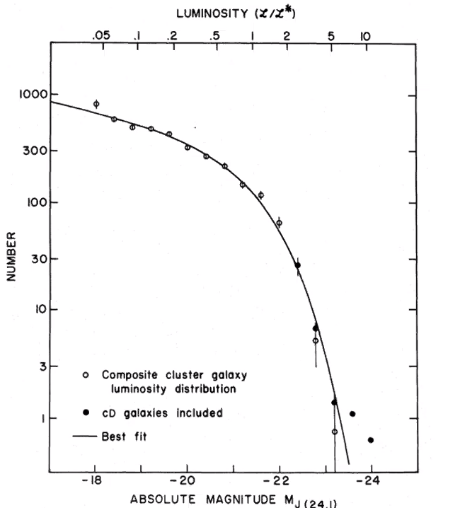
\includegraphics[height=0.5\textwidth]{images/luminosity_function.png}}
\end{itemize}
\subsection{The K-Correction}
\begin{itemize}
    \item De-redshift
    \item K-correction ``corrects'' for the fact that sources observed at different redshifts are compared with each other at different rest wavelength bands
    \item Calculating the absolute magnitude of galaxies requires making corrections to their observed apparent magnitudes if we are to properly account for the effect of extinction, both within the Milky Way and within the target galaxy.
\end{itemize}
\section{Galactic Evolution}
\subsection{Major versus Minor Galaxy Mergers}
\begin{itemize}
    \item Major merger: mass ratio of merging galaxies is between 3:1 and 1:1
    \item Minor merger: mass ratio of merging galaxies is below 3:1
\end{itemize}
\subsection{Tidal Stripping and Tidal Tails}
\begin{itemize}
    \item Tidal stripping: $$F = \frac{2 G M m R}{r^3}$$ where $F$ is the tidal force on the galaxy of mass $m$, has radius $R$, and is a distance $r$ from a galaxy with mass $M$.
    \item Tidal tails are a result of tidal stripping as the tidal forces unbind gas and stars from galaxies
    \item The Milky Way is currently stripping material from the Large and Small Magellanic Clouds!
\end{itemize}
\subsection{Dynamical Friction}
\begin{itemize}
    \item As an object of mass $M$ moves through a galaxy, a high-density ``wake'' forms behind it. This wake exerts net gravitational force on $M$ that opposes its forward motion, slowing it down.
          \begin{itemize}
              \item This is the reason for mergers, otherwise objects would just pass through each other.
          \end{itemize}
    \item Force due to dynamical friction is given by $$F_d = - 4 \pi \ln(\Lambda) \left( \frac{G^2 M^2 \rho}{v^2} \right)$$ where $\Lambda = b_{max}/m_{min}$ (depends on the material/density of material the galaxy is moving through) and $\rho = n m$
    \item In class, we assumed the density of the dark matter halo to be $$\rho (r) = \frac{v^2}{4 \pi G r^2}$$
\end{itemize}
\subsection{Initial Mass Function}
\begin{itemize}
    \item Only gives distribution of stellar masses immediately after stars are born (doesn't give mass distribution of, for example, stars in the Milky Way today).
    \item $$\xi (M) = \frac{dN}{dM} = C M^{-(1 + x)}$$ where $N$ is the number of stars, $M$ is the mass of the stars, and $C$ is a normalization constant. For stars with masses in the range $7 M_\odot < M < 35 M_\odot$, $x = 1.8$.
    \item The above leads directly to $$N = \int_0^\infty \xi (M)\ dM$$ for \emph{all} masses (change bounds for given range).

          \centering{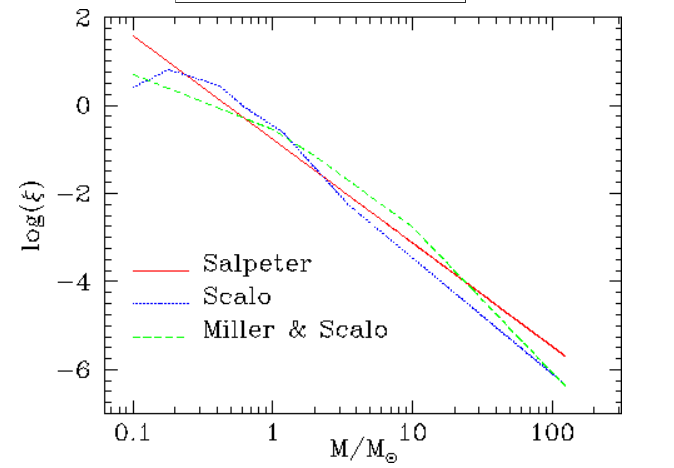
\includegraphics[height=0.5\textwidth]{images/imf.png}}
\end{itemize}
\subsection{Eggen, Lynden-Bell, and Sandage Collapse Model}
\begin{itemize}
    \item Galaxy forms all at once from direct collapse of a proto-galactic nebula
    \item ``Top-down'' model
\end{itemize}
\subsection{Hierarchical Merger Model}
\begin{itemize}
    \item Stars in the stellar halo were a part of stellar clusters in initial proto-galaxies (some clusters survived to become globular clusters)
    \item Proto-galactic gas clouds collided and settled toward the center, forming a thick disk
    \item Gas continued to settle onto the midplane, forming a thin disk
    \item Stripped gas from satellite galaxies in recent mergers settled toward the galactic center accounting for the young stars in the bulge
    \item ``Bottom-up'' model: small galaxies merge to larger galaxies
    \item Future gas for bulge: tidal stripping of LMC and SMC
\end{itemize}
\subsubsection{Galaxy Structure}
\begin{enumerate}
    \item \textbf{Globular Clusers and Stellar Halos:} stellar clusters formed in proto-galaxies and merged to form galaxies. Some stars tidally got stipped away to become stars of stellar halo and some stellar clusters survived to become globular clusters.
    \item \textbf{Thick Disk:} proto-galactic gas clouds collided and settled towards the center of the galaxy and then cooled to form new stars
    \item \textbf{Thin Disk:} After the thick disk formation, gas continued to settle onto a galactic midplane and formed new stars
    \item \textbf{Young Stars in the Bulge:} recent mergers with satellite galaxies stripped gas and settled towards the galactic center
    \item \textbf{Future Gas for the Bulge:} tidal stripping of LMC and SMC
\end{enumerate}
\subsubsection{Morphology-Density Relation}
Due to more mergers occurring in dense environments (clusters) and the transformation of spirals into ellipticals during mergers, elliptical galaxies are more abundant in clusters.
\subsubsection{Butcher-Oemler Effect}
\begin{itemize}
    \item Galaxies becoming redder over time
    \item If a $z = 0$ galaxy cluster has 40\% ellipticals, a $z = 2$ galaxy cluster has $< 40\%$ ellipticals and more blue spirals. Note: redshift of 2 corresponds to most merger events

          \centering{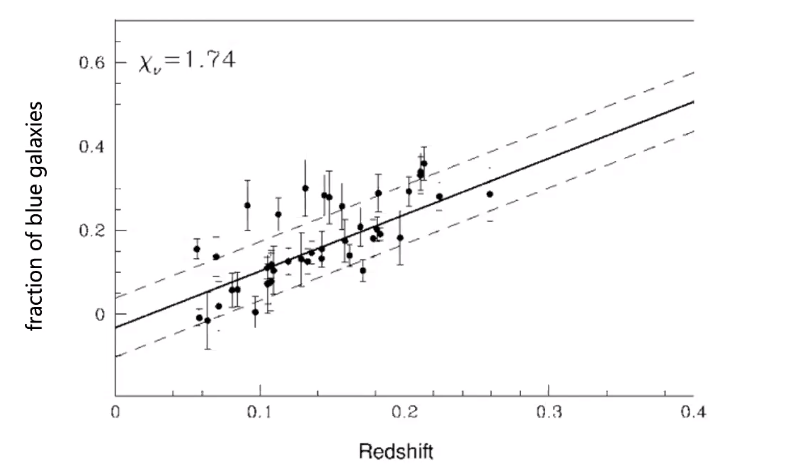
\includegraphics[height=0.5\textwidth]{images/boe.png}}
\end{itemize}
\section{The Structure of the Universe}

\subsection{The Cosmological Distance Ladder}

\begin{center}
    {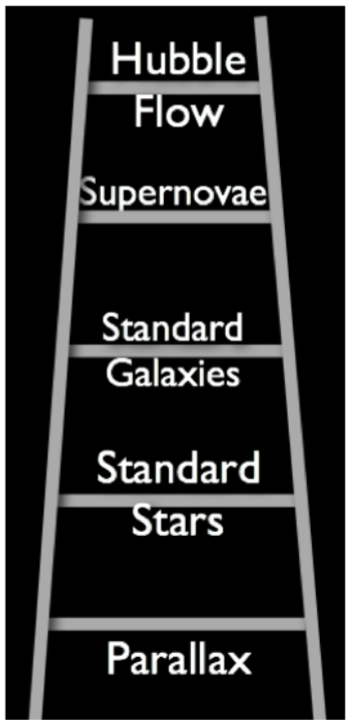
\includegraphics[height=0.5\textwidth]{images/stuct_uni.png}}
\end{center}

\subsubsection{Parallax}
\begin{itemize}
    \item Only out to one kiloparsec

          \begin{center}
              {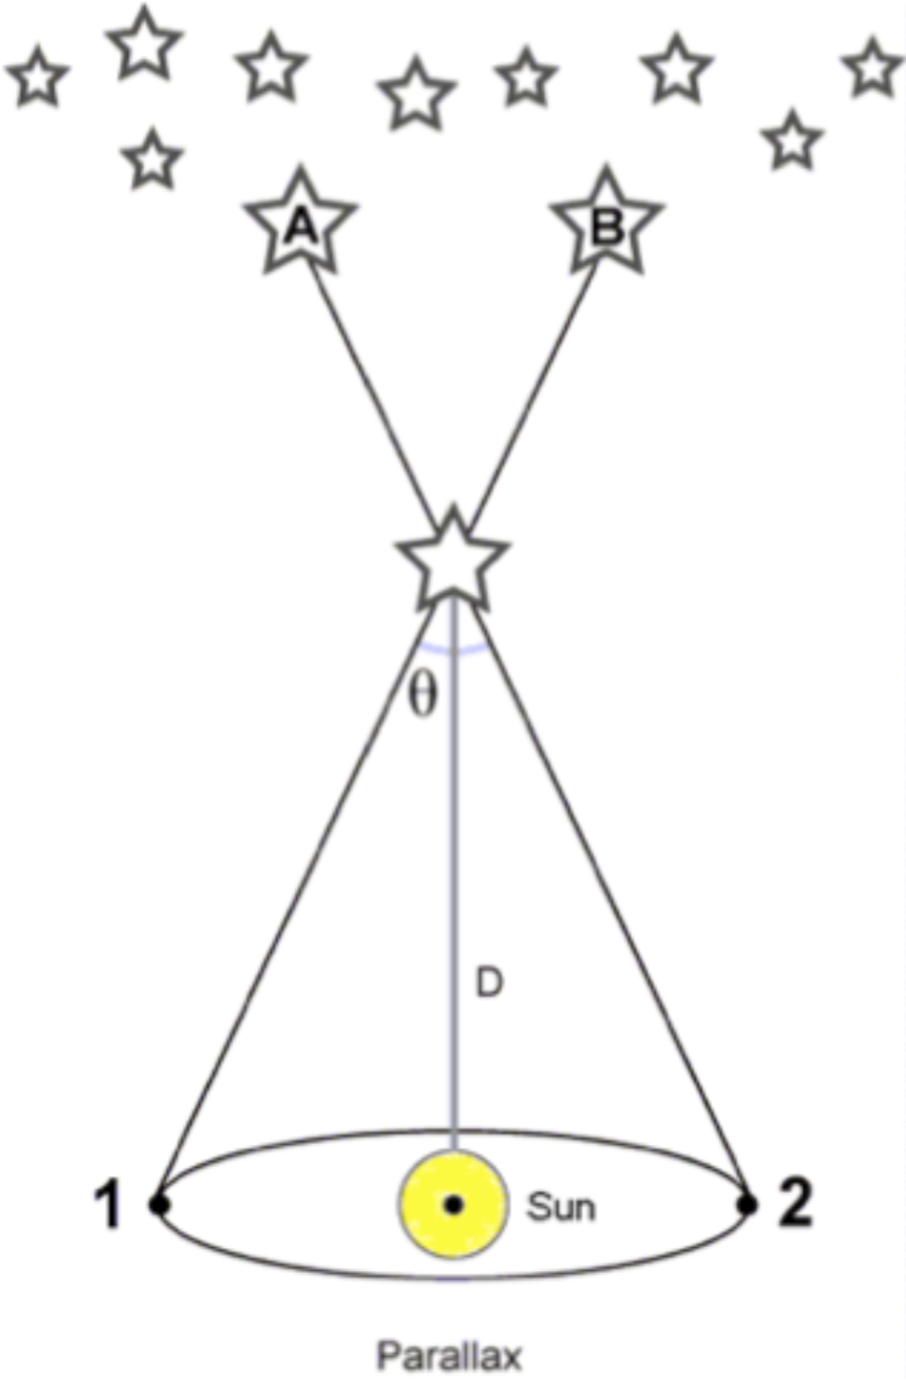
\includegraphics[height=0.5\textwidth]{images/parallax.png}}
          \end{center}

\end{itemize}
\subsubsection{Cepheid Variable Stars}
\begin{itemize}
    \item Out to 30 Mpc
    \item Cepheids pulsate rapidly and we can measure the period of pulsations
    \item Period-luminosity relationship for Cepheids: $$M_V = -3.53 \log (P_d) - 2.13 + 2.13(B-V)$$ where $M_V$ is the absolute visual magnitude, $P_d$ is the period in days, and $B - V$ is the color index.
    \item What can we find?
          \begin{itemize}
              \item Observe $P_d$ and $B - V$, infer $M_V$
              \item Observe $m_V$, use $M_V$ from above to get distance ($d = 10^{(m - M + 5)/5}$ parsecs)
          \end{itemize}
    \item Notes: Blue Cepheids are brighter, longer period means brighter
\end{itemize}
\subsubsection{Tully-Fisher Relation}
\begin{itemize}
    \item Out to 100 Mpc
    \item Only works for spiral galaxies
    \item What can we find?
          \begin{itemize}
              \item Observe $v_{max}$ (distance between center and peak of graph), infer $M_B$
              \item Observe $m_B$, infer distance
          \end{itemize}
\end{itemize}
\subsubsection{Supernovae}
\begin{itemize}
    \item Out to $> 1000 Mpc$
    \item Measure the size of a nearby supernova's photosphere

          \begin{center}
              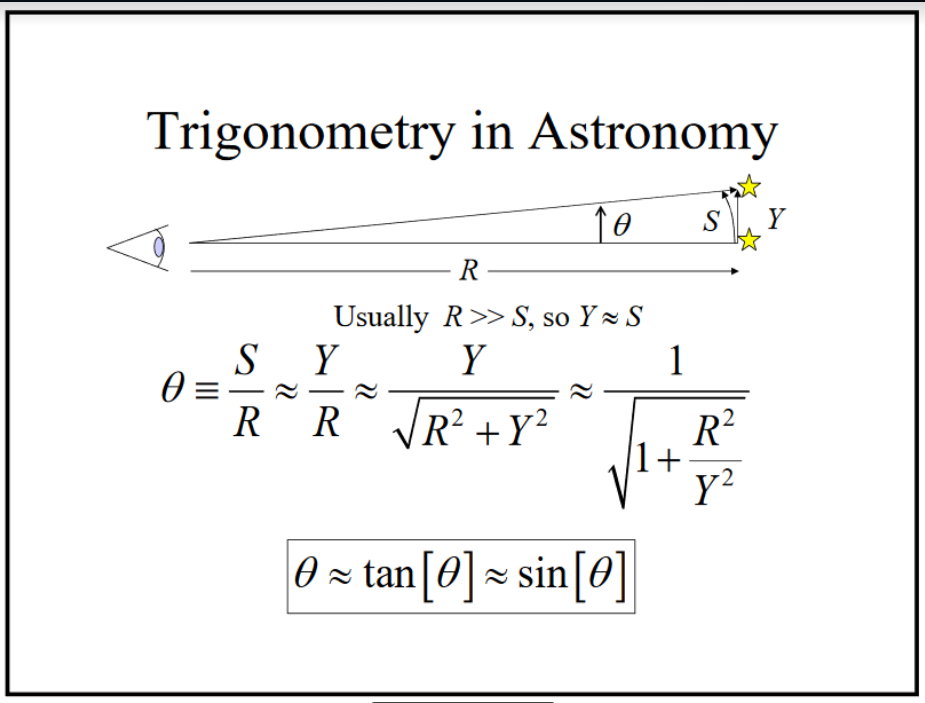
\includegraphics[height=0.5\textwidth]{images/trig_astro.png}
          \end{center}

    \item Type Ia light curves:
          \begin{itemize}
              \item The maximum brightness of a supernova is inversley correlated with the rate of light curve decline (bright supernovae decline more slowly)
              \item What can we find?
                    \begin{itemize}
                        \item Observe rate of decline, infer $M$
                        \item Observe $m$, combine with peak $M$ to get distance
                    \end{itemize}
          \end{itemize}
\end{itemize}
\subsubsection{Hubble Flow}
\begin{itemize}
    \item Most galaxies exhibit redshifts in their spectra: $v = cs$ for $v \ll c$.
          \begin{itemize}
              \item Farther galaxy means larger redshift means moving faster means ``Hubble flow''
          \end{itemize}
    \item Hubble's Law: $v = H_0 d$ where $v$ is the galaxy's velocity along the line of sight, $d$ is the distance to the galaxy in Mpc, and $H_0$ is Hubble's constant (current value of 71 km/sec/Mpc - controversial)
    \item Highest rung on the distance ladder - most galaxies
          \begin{center}
              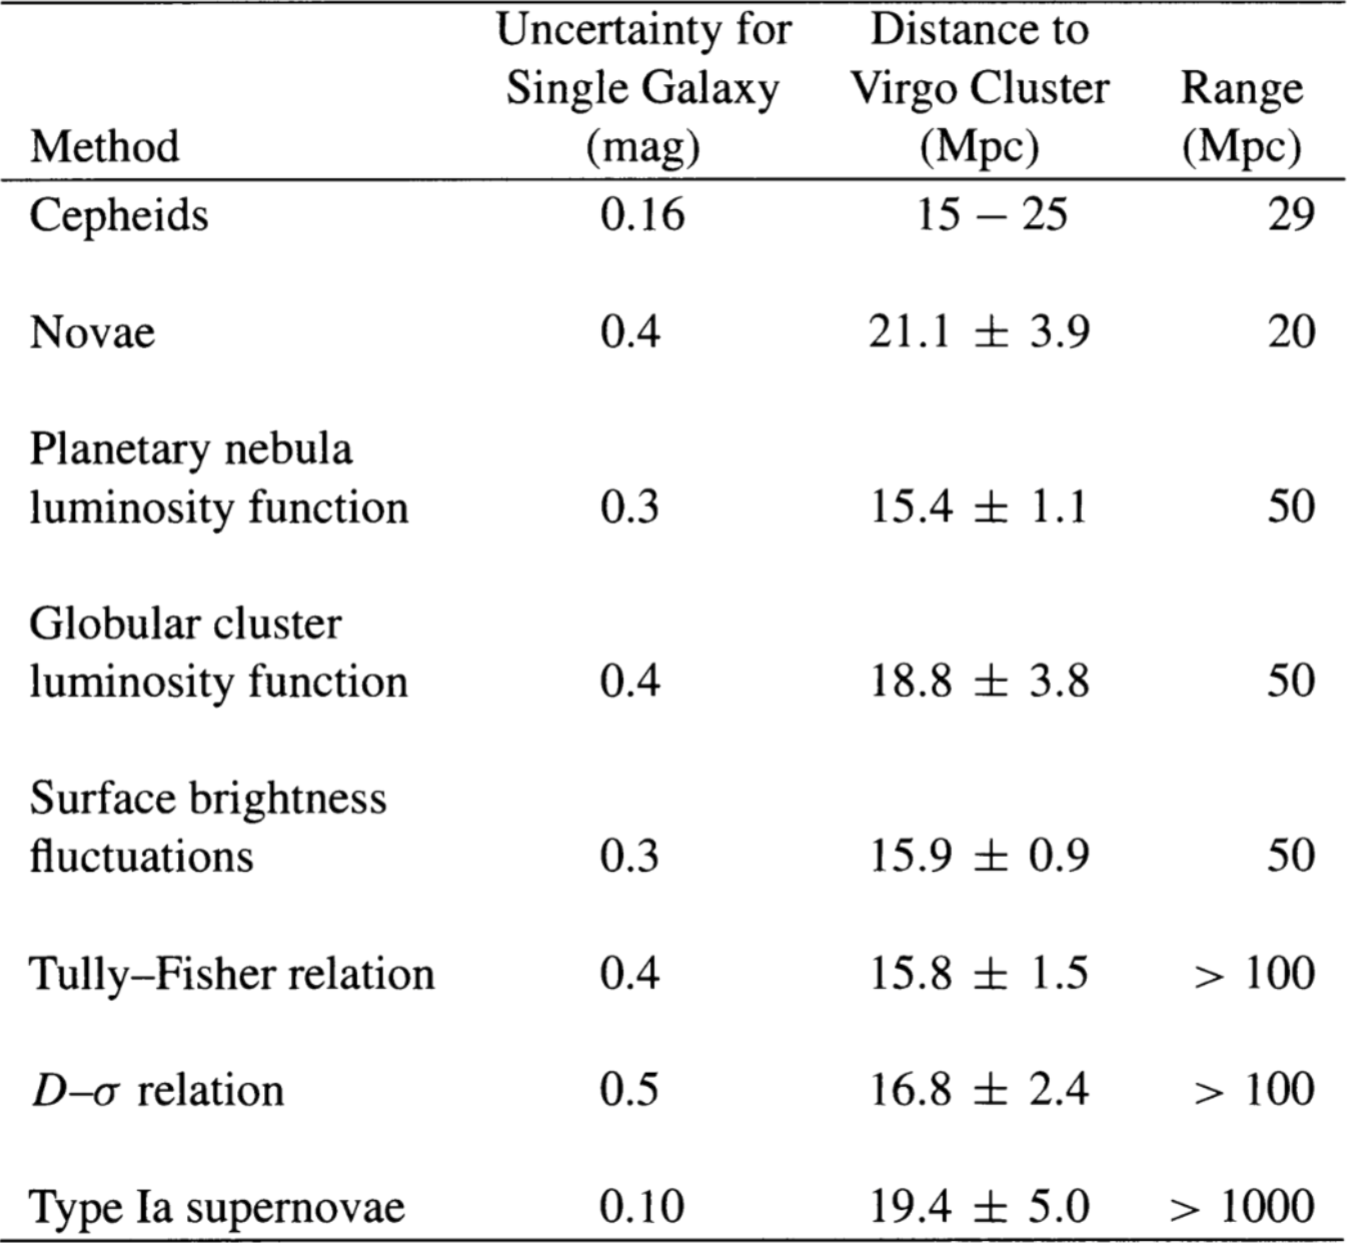
\includegraphics[width=0.5\textwidth]{images/dist_ladd.png}
          \end{center}
\end{itemize}
\subsection{Expanding Universe, Hubble's Law}
\begin{itemize}
    \item The further a galaxy is from Earth, the fast it is moving away and the larger its redshift $z$
    \item For non-relativistic motion: $$z = \frac{\lambda_{obs} - \lambda_{rest}}{\lambda_{rest}} = \frac{v}{c}$$
    \item For relativistic motion: $$z = \sqrt{\frac{1 + v/c}{1 - v/c}} - 1 \to \frac{v}{c} = \frac{(z+1)^2 - 1}{(z+1)^2 + 1}$$
    \item Hubble's Law $v = H_0 d$ where $H_0$ is the Hubble constant. $H_0 = 100 h$ km/s/Mpc
    \item Most galaxies are red-shifted and moving away, but some are blue-shifted, for example, Andromeda (M31)
\end{itemize}
\subsection{Peculiar Velocity}
\begin{itemize}
    \item A galaxy's own velocity through space (as opposed to recessional velocity which is the velocity of the expanding universe carrying the galaxy along)
    \item If the recessional velocity is less than the peculiar velocity, the object is coming towards you!
\end{itemize}
\subsection{The Age of the Universe}
\begin{itemize}
    \item Assume constant rate of expansion
    \item $t = d/v = d / (H_0 \times d) = 1 / H_0$
    \item Gives estimate of around 13 billion years which isn't too far off!
\end{itemize}
\subsection{Distribution of Galaxies in the Universe}
\begin{itemize}
    \item More ellipticals near center of galaxy cluster due to being more dense and more likely for galaxies to merge and form ellipticals
    \item More likely for spiral galaxies to be on outer edge where mergers less likely
    \item Spirals more abundant in field, ellipticals more abundant in clusters
          \begin{center}
              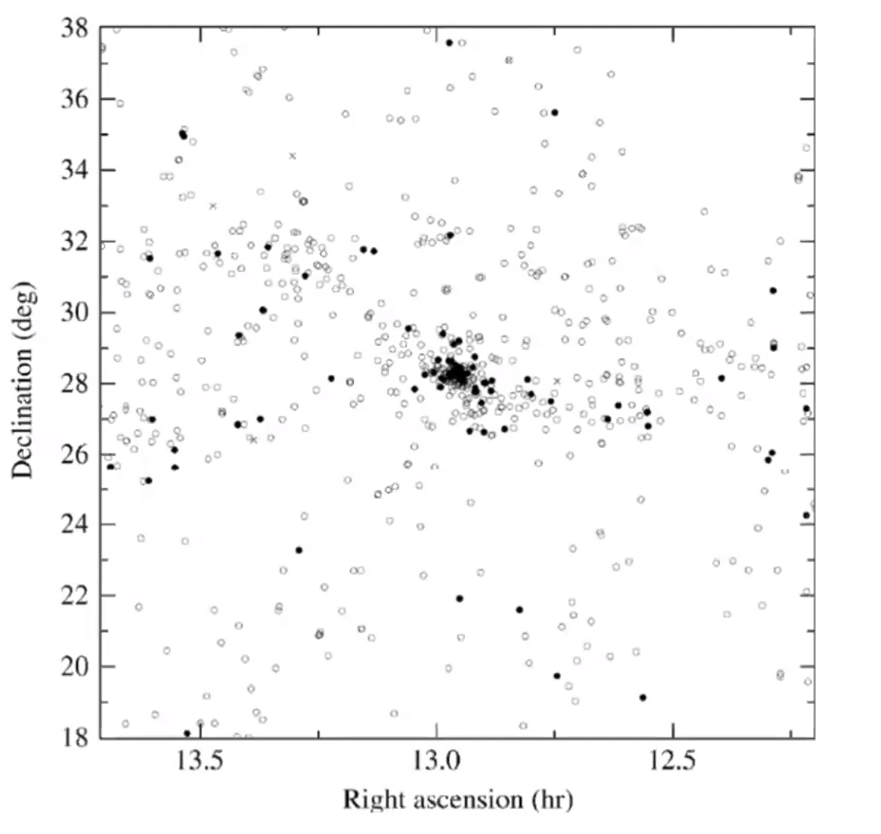
\includegraphics[height=0.5\textwidth]{images/distro_galax.png}
          \end{center}
\end{itemize}
\subsection{Groups and Cluster}
\begin{itemize}
    \item Most galaxies are found in groups or clusters: gravitationally bound associations of galaxies
    \item Groups have less than 50 members, diameter $1.4 h^{-1}$ Mpc, velocity dispersion 150 km/s, and mass $2 \times 10^{13} h^{-1} M_\odot$.
    \item Clusters have between 50 and 1000 members (poor to rich, respectively) with diameter $6 h^{-1}$ Mpc, velocity dispersion between 800 and 1000 km/s, and mass $10^{15} M_\odot$.
          \begin{center}
              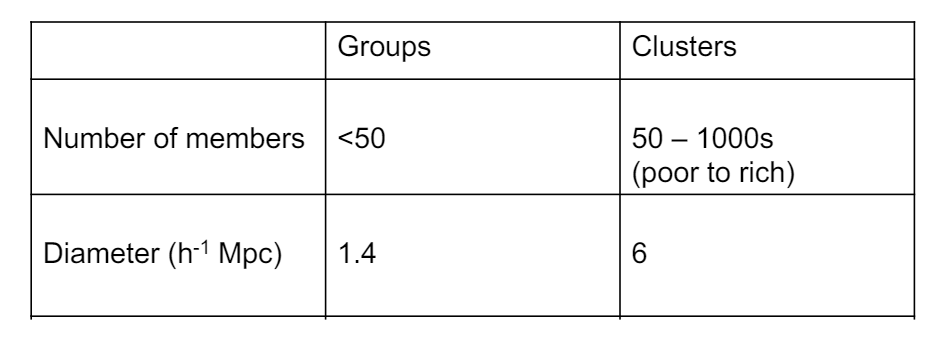
\includegraphics[width=0.5\textwidth]{images/table.png}
          \end{center}
    \item Local Group: Milky Way and Andromeda, M33, and Pinwheel galaxy
    \item Nearest galaxy clusters:
          \begin{itemize}
              \item Virgo Cluster: 16 Mpc away, 250 larger galaxies, 2000 smaller galaxies, diameter 3 Mpc
              \item Coma Cluster: 90 Mpc away, roughly 10000 member galaxies, diameter 6 Mpc
          \end{itemize}
    \item There are more elliptical galaxies at the center of a galaxy cluster
    \item Virial Mass for a galaxy cluster (lecture 12 boardwork): $$M = \frac{5 R \sigma^2}{G}$$
\end{itemize}
\subsection{Evidence for Dark Matter from Cluster Masses}
\begin{itemize}
    \item Fritz ``Nuclear Goblins Guy'' Zwicky measured the velocity dispersion and estimated the cluster mass
    \item Compared to the total mass of galaxies in the cluster
    \item Total mass of galaxies did not account for all the mass in the cluster
    \item ``Missing mass'' turned out to be dark matter and hot intracluster gas
\end{itemize}
\subsection{Intracluster Gas}
\begin{itemize}
    \item Roughly 90\% of the baryonic mass of a galaxy cluster is in the form of ionized gas
    \item Gas radiates via thermal bremsstrahlung: free-free emission of x-ray photons
    \item Using ideal gas law and HSE, can derive galaxy cluster mass as a function of r entirely from hot intracluster gas quantities: $$M_r = - \frac{k T r}{\mu m_H G} \left( \frac{\partial \ln \rho}{\partial \ln r} + \frac{\partial \ln T}{\partial \ln r}\right)$$ where $\mu$ is a constant.
    \item To find the total mass, evaluate $M_r (r = R)$.
    \item The hotter the gas, the more massive the cluster.
\end{itemize}
\chapter{Final Exam Content}
\section{Active Galaxies}
\subsection{Active Galactic Nuclei}
\begin{itemize}
    \item Active Galactic Nuclei: Supermassive black holes that are active/accreting gas (most of them are inactive). Their host galaxy is called an Active galaxy
          \begin{itemize}
              \item FYI: never put your nose across the event horizon boundary
                    \begin{center}
                        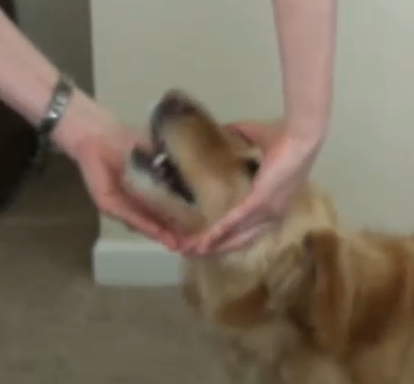
\includegraphics[width = 0.2\textwidth]{images/agn_dog.png}
                    \end{center}
              \item Calculating if another galaxy has a SMBH by measuring spectra of the gas at the center, get a velocity map and calculate the mass
          \end{itemize}
    \item Types:
          \begin{itemize}
              \item Quasars
                    \begin{itemize}
                        \item Quasi-stellar radio sources
                        \item Very luminous (most luminous AGN) and visible from far away
                        \item Have both broad and narrow emission lines in their spectra
                        \item Quasars are radio-loud, QSOs are radio-quiet
                        \item Their energy comes from accretion onto supermassive black holes
                        \item Even 1 solar mass of accreting gas can generate enough energy to outshine the galaxy
                        \item To find out if a source is a star or an AGN, look at the spectra
                    \end{itemize}
              \item Seyferts
                    \begin{itemize}
                        \item Most common types of AGNs (weaker AGN)
                        \item Usually found in spiral galaxies
                        \item Defined by their spectra:
                              \begin{itemize}
                                  \item Type 1 Seyfert: has both broad and narrow emission lines
                                  \item Type 2 Seyfert: has narrow emission lines only
                              \end{itemize}
                    \end{itemize}
              \item Radio Galaxies
                    \begin{itemize}
                        \item Have strong radio emission (from synchrotron radiation)
                        \item Usually found in elliptical galaxies
                        \item Two categories:
                              \begin{itemize}
                                  \item BLRG = broad and narrow emission lines
                                  \item NLRG = narrow emission lines only
                              \end{itemize}
                        \item Radio jets
                    \end{itemize}
              \item Blazars
                    \begin{itemize}
                        \item Have almost no emission lines
                        \item Strong radio emission
                        \item Usually found in elliptical galaxies
                    \end{itemize}
          \end{itemize}
          \begin{center}
              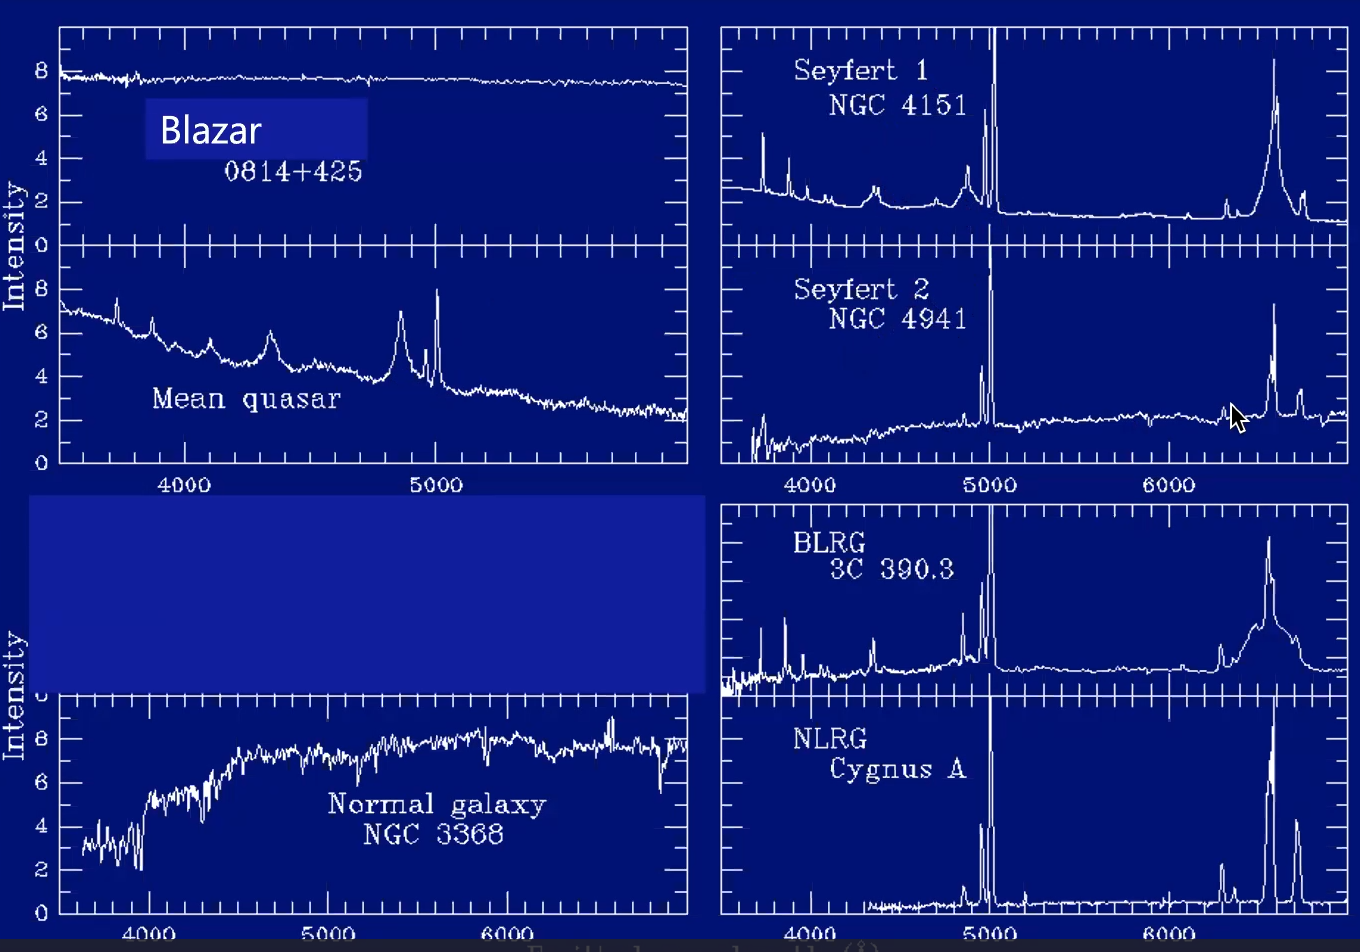
\includegraphics[height = 0.6 \textwidth]{images/types_agn.png}
          \end{center}
\end{itemize}
\subsection{AGN Structure}
\begin{center}
    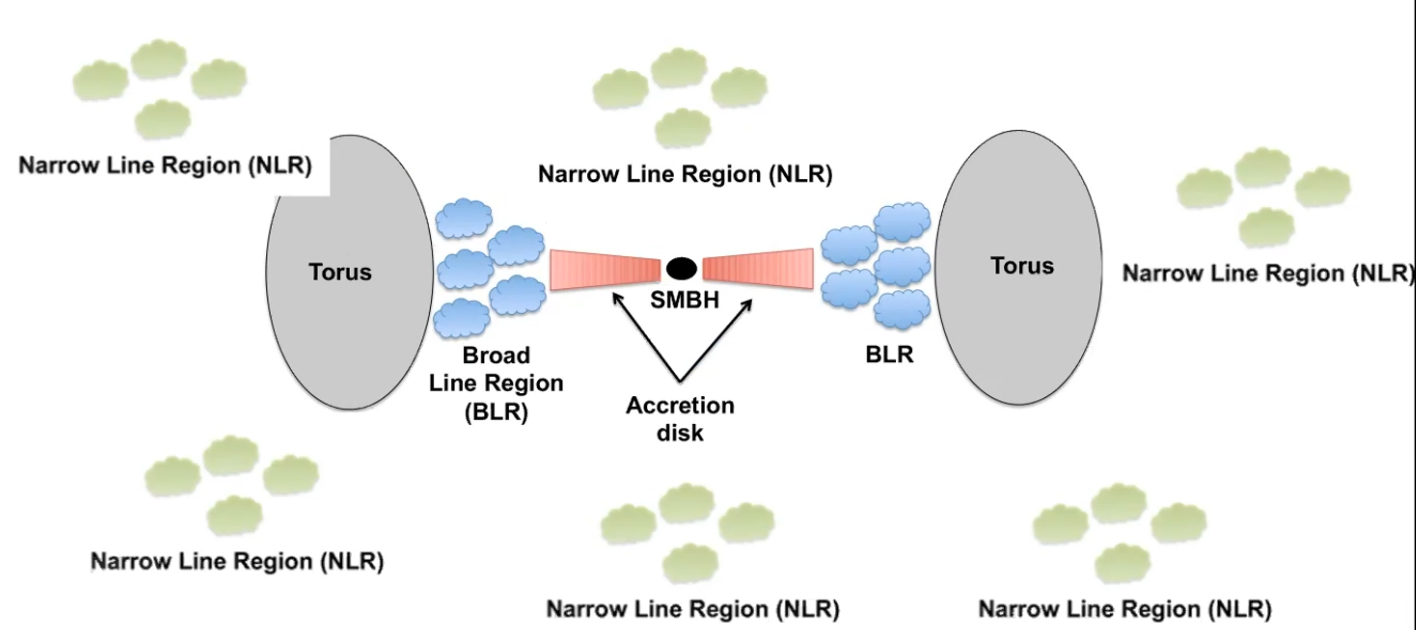
\includegraphics[width = \textwidth]{images/agn_structure.png}
\end{center}
More specifics on how this works and what angles to see, etc. in Lecture 16, slides 6-10.
\subsection{AGN Luminosity}
\begin{itemize}
    \item Accretion luminosity:
          \begin{equation*}
              L_{disk} = \eta \dot{M} c^2 \tag{C\&O 28.6}
          \end{equation*}
          where $\eta$ is the efficiency of the process, usually aroun 10\%.
    \item Not all the energy of the accretion disk goes into luminosity, some goes into heat
    \item There is an upper limit to the luminosity you can get: the Eddington Luminosity Limit is given by
          \begin{equation*}
              L_{Ed} = \frac{4 \pi G c}{\bar{\kappa}} M  \simeq 1.5 \times 10^{31} \frac{M}{M_\odot}\ W \tag{10.114}
          \end{equation*}
          and represents the maximum radiative luminosity that a star can have and still remain in hydrostatic equilibrium.
\end{itemize}
\subsubsection{AGN Variability}
\begin{itemize}
    \item Luminosity can vary on timescales as short as months, weeks or days
    \item Broad emission lines are variable but narrow emission lines have little variation
    \item Calculate the size of the Broad Line Region (BLR), using the timescale of variability: $d = c \Delta t$
          \begin{center}
              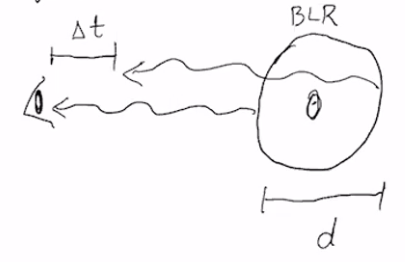
\includegraphics[height = 0.3 \textwidth]{images/broad_line.png}
          \end{center}
    \item Calculate the size of the Narrow Line Region (NLR), using the Stromgren radius:
          \begin{equation*}
              r_{NLR} \approx \left( \frac{3N}{4 \pi \alpha_{qm} \epsilon} \right)^{1/3} \frac{1}{n_e^{2/3}} \tag{C\&O 28.13}
          \end{equation*}
    \item Flickering AGN (burping): supermassive black hole that accretes some gas (became an AGN), and created radiation. Then the AGN stopped accreting, then later on it started accreting gas again. Caused by galaxy mergers. Fermi bubble: echo from Sgr A$^*$.
    \item Voorwerp: echos of emission from an AGN that has since turned off
    \item Spectral Energy Distribution (SED) of an AGN: spectrum that covers all wavelengths
          \begin{itemize}
              \item Radio: radio-loud and radio quiet AGN
              \item IR bump: reradiated light from the dusty torus
              \item Big blue bump: in UV, direct thermal emission from all the gas in the accretion disk
              \item X-ray: Compton scattering of the accretion disk photons
          \end{itemize}
    \item Monochromatic Energy Flux: AGN can be approximated by
          \begin{equation*}
              F_\nu \propto \nu^{-\alpha} \tag{C\&O 28.1}
          \end{equation*}
\end{itemize}
\subsection{Gravitational Lensing}
\begin{itemize}
    \item Massive objects warp spacetime, more massive, more curved
    \item Gravitational wave:
          \begin{itemize}
              \item Any massive object rolling around creates gravitational waves
              \item Gravitational waves stretch and compress Earth as they pass by
              \item LIGO has detected 70 mergers
              \item LISA to detect gravitational waves in space using laser interferometry between three free-flying spacecraft
          \end{itemize}
    \item Gravitational Lensing
          \begin{center}
              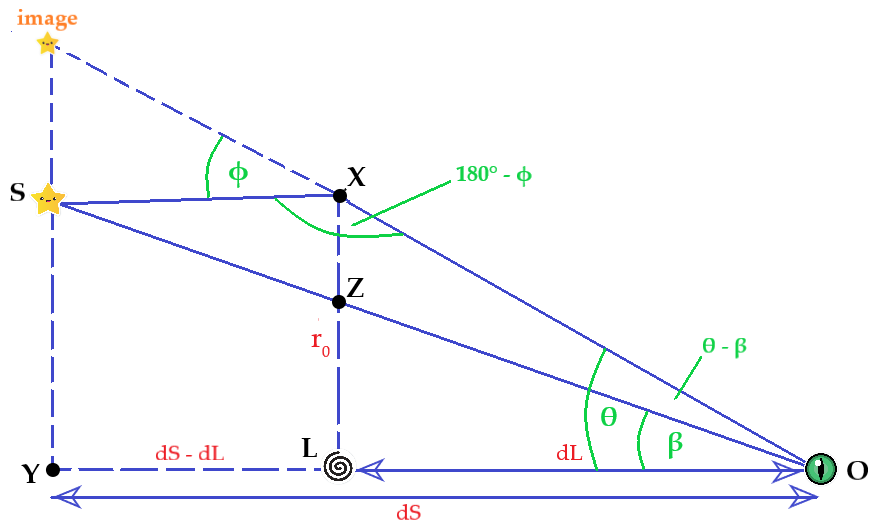
\includegraphics[height = 0.4 \textwidth]{images/lensing.png}
          \end{center}
          \begin{itemize}
              \item Light from a background source traveling through curved space-time near a massive lens can create multiple observed images of the source. The angular deviation of a photon passing a distance $r_0$ from a mass $M$ is
                    \begin{equation*}
                        \phi = \frac{4 G M}{r_0 c^2}\ \text{rad} \tag{C\&O 28.20}
                    \end{equation*}
              \item Lens equation:
                    \begin{equation*}
                        \theta^2 - \beta \theta - \frac{4 G M}{c^2} \left( \frac{d_s - d_L}{d_s d_L} \right) = 0 \tag{C\&O 28.21}
                    \end{equation*}
              \item Mass of the lens:
                    \begin{equation*}
                        M = - \frac{\theta_1 \theta_2 c^2}{4 G} \left( \frac{d_S d_L}{d_S - d_L} \right) \tag{C\&O 28.23}
                    \end{equation*}
              \item Einstein ring: when the source is exactly behind the lens, it creates a perfect circle around the lens
                    \begin{equation*}
                        \theta_E = \sqrt{\frac{4 G M}{c^2} \left( \frac{d_S - d_L}{d_S d_L} \right) }\ \text{rad} \tag{C\&O 28.24}
                    \end{equation*}
              \item Uses of gravitational lensing:
                    \begin{itemize}
                        \item Measure masses of lenses (assuming a NFW profile)
                        \item Search for dark matter via MACHO lensing (microlensing)
                    \end{itemize}
              \item Regimes
                    \begin{itemize}
                        \item Microlensing: lens not very massive (i.e. MACHOs), flickering
                        \item Strong lensing: lens is massive
                        \item Weak lensing: multiple images not produced, instead tiny distortion of the shape of the object
                    \end{itemize}
          \end{itemize}
\end{itemize}
\section{Cosmology}
Cosmological principle: the universe is isotropic and homogeneous.
\subsection{Models}
\subsubsection{Pressureless Dust Model}
\begin{itemize}
    \item Only one component: pressureless dust
          \begin{center}
              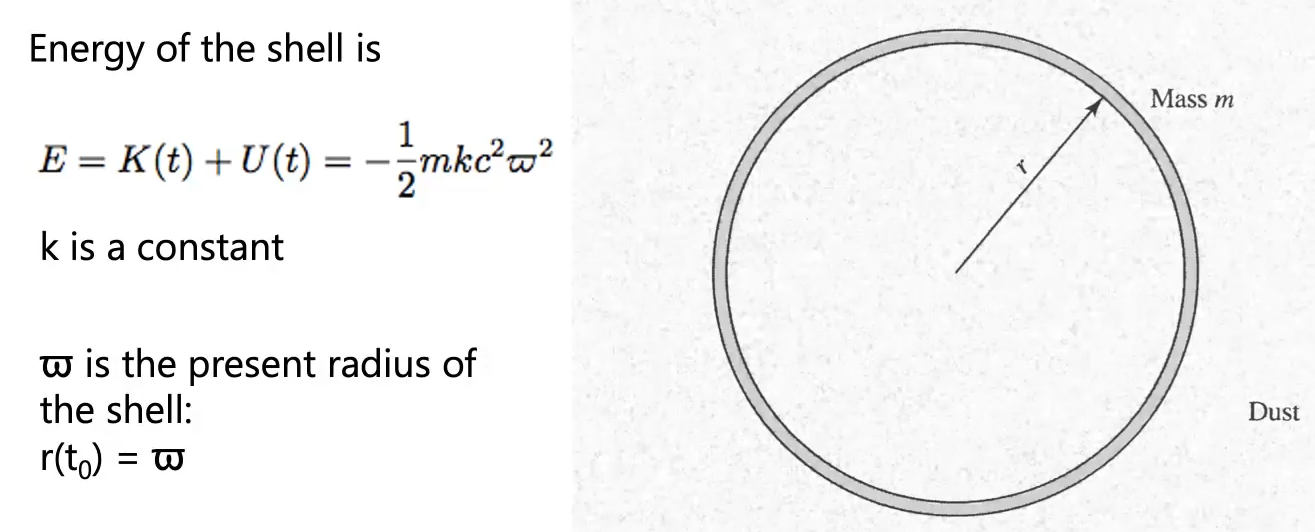
\includegraphics[width = 0.9 \textwidth]{images/cosmo_setup.png}
          \end{center}
    \item $\varpi$ is the co-moving coordinate
    \item For $k > 0$, $\Omega_0 > 1$, universe is closed and will collapse on itself
    \item For $k < 0$, $\Omega_0 < 1$, universe is open and will expand forever
    \item For $k = 0$, $\Omega_0 = 1$, universe is flat and will slow down and come to a halt as $t \to \infty$
    \item $R(t)$ is the scale factor that describes the expansion (dimensionless)
          \begin{equation*}
              r(t) = R(t) \varpi \tag{C\&O 29.3}
          \end{equation*}
    \item $R$ and the redshift $z$ are related by
          \begin{equation*}
              R = \frac{1}{1 + z} \tag{C\&O 29.4}
          \end{equation*}
    \item Today, $R = 1$ ($z = 0$). At $z = 2$, the size of the universe was $\frac{1}{3}$ what it is today.
    \item Hubble Law:
          \begin{equation*}
              v(t) = H(t) r(t) = H(t) R(t) \varpi \tag{C\&O 29.7}
          \end{equation*}
    \item The value of the density that will result in a value of $k = 0$ is known as the critical density,
          \begin{equation*}
              \rho_c (t) = \frac{3 H^2 (t)}{8 \pi G} \tag{C\&O 29.12}
          \end{equation*}
    \item The density parameter $\Omega (t)$ is the ratio of a measured density to the critical density:
          \begin{equation*}
              \Omega_0 = \frac{\rho_0}{\rho_c} = \frac{8 \pi G \rho_0}{3 H_0^2}
          \end{equation*}
    \item For a flat universe ($k = 0$, $\rho_0 = \rho_{c,0}$, and $\Omega_0 = 1$),
          \begin{equation*}
              R_{flat} = \left( \frac{3}{2} \right)^{2/3} \left( \frac{t}{t_H} \right)^{2/3} \tag{C\&O 29.31}
          \end{equation*}
          \begin{itemize}
              \item the universe was essentially flat
          \end{itemize}
\end{itemize}
\subsubsection{Two-Component Model}
\begin{itemize}
    \item Accounts for the relativistic equivalence of mass and energy from CMB on expansion
    \item Includes both the total density of matter (baryonic and dark), $\rho_m$, and the equivalent mass density of relativistic particles (such as neutrinos and CMB photons), $\rho_{rel}$
    \item Equation of state:
          \begin{equation*}
              P = w u \tag{C\&O 29.52}
          \end{equation*}
          \begin{itemize}
              \item matter: $w_m = 0$
              \item relativistic particle: $w_{rel} = 1/3$
              \item dark energy: $w_\Lambda = -1$
          \end{itemize}
    \item Density evolves as
          \begin{equation*}
              R^{3(1 + w)} \rho = \text{constant} = \rho_0
          \end{equation*}
\end{itemize}
\subsubsection{Three-Component ($\Lambda$CDM) Model}
See Early Universe section below.
\subsection{Cosmic Microwave Background}
\begin{center}
    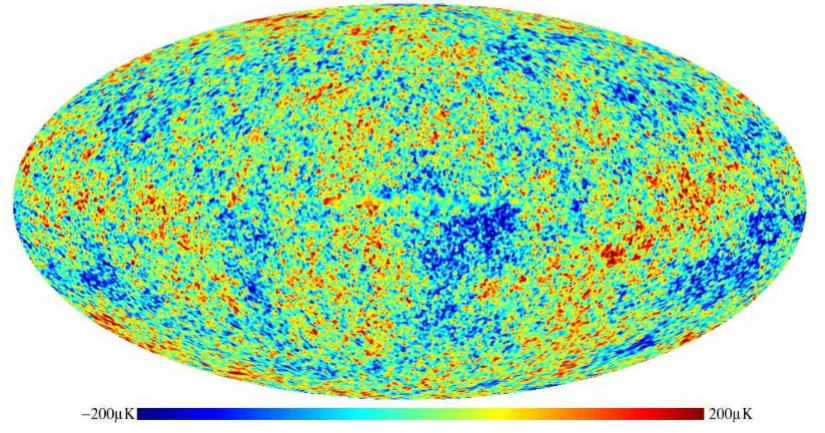
\includegraphics[height = 0.4 \textwidth]{images/CMB.png}
\end{center}
\begin{itemize}
    \item Temperature
          \begin{center}
              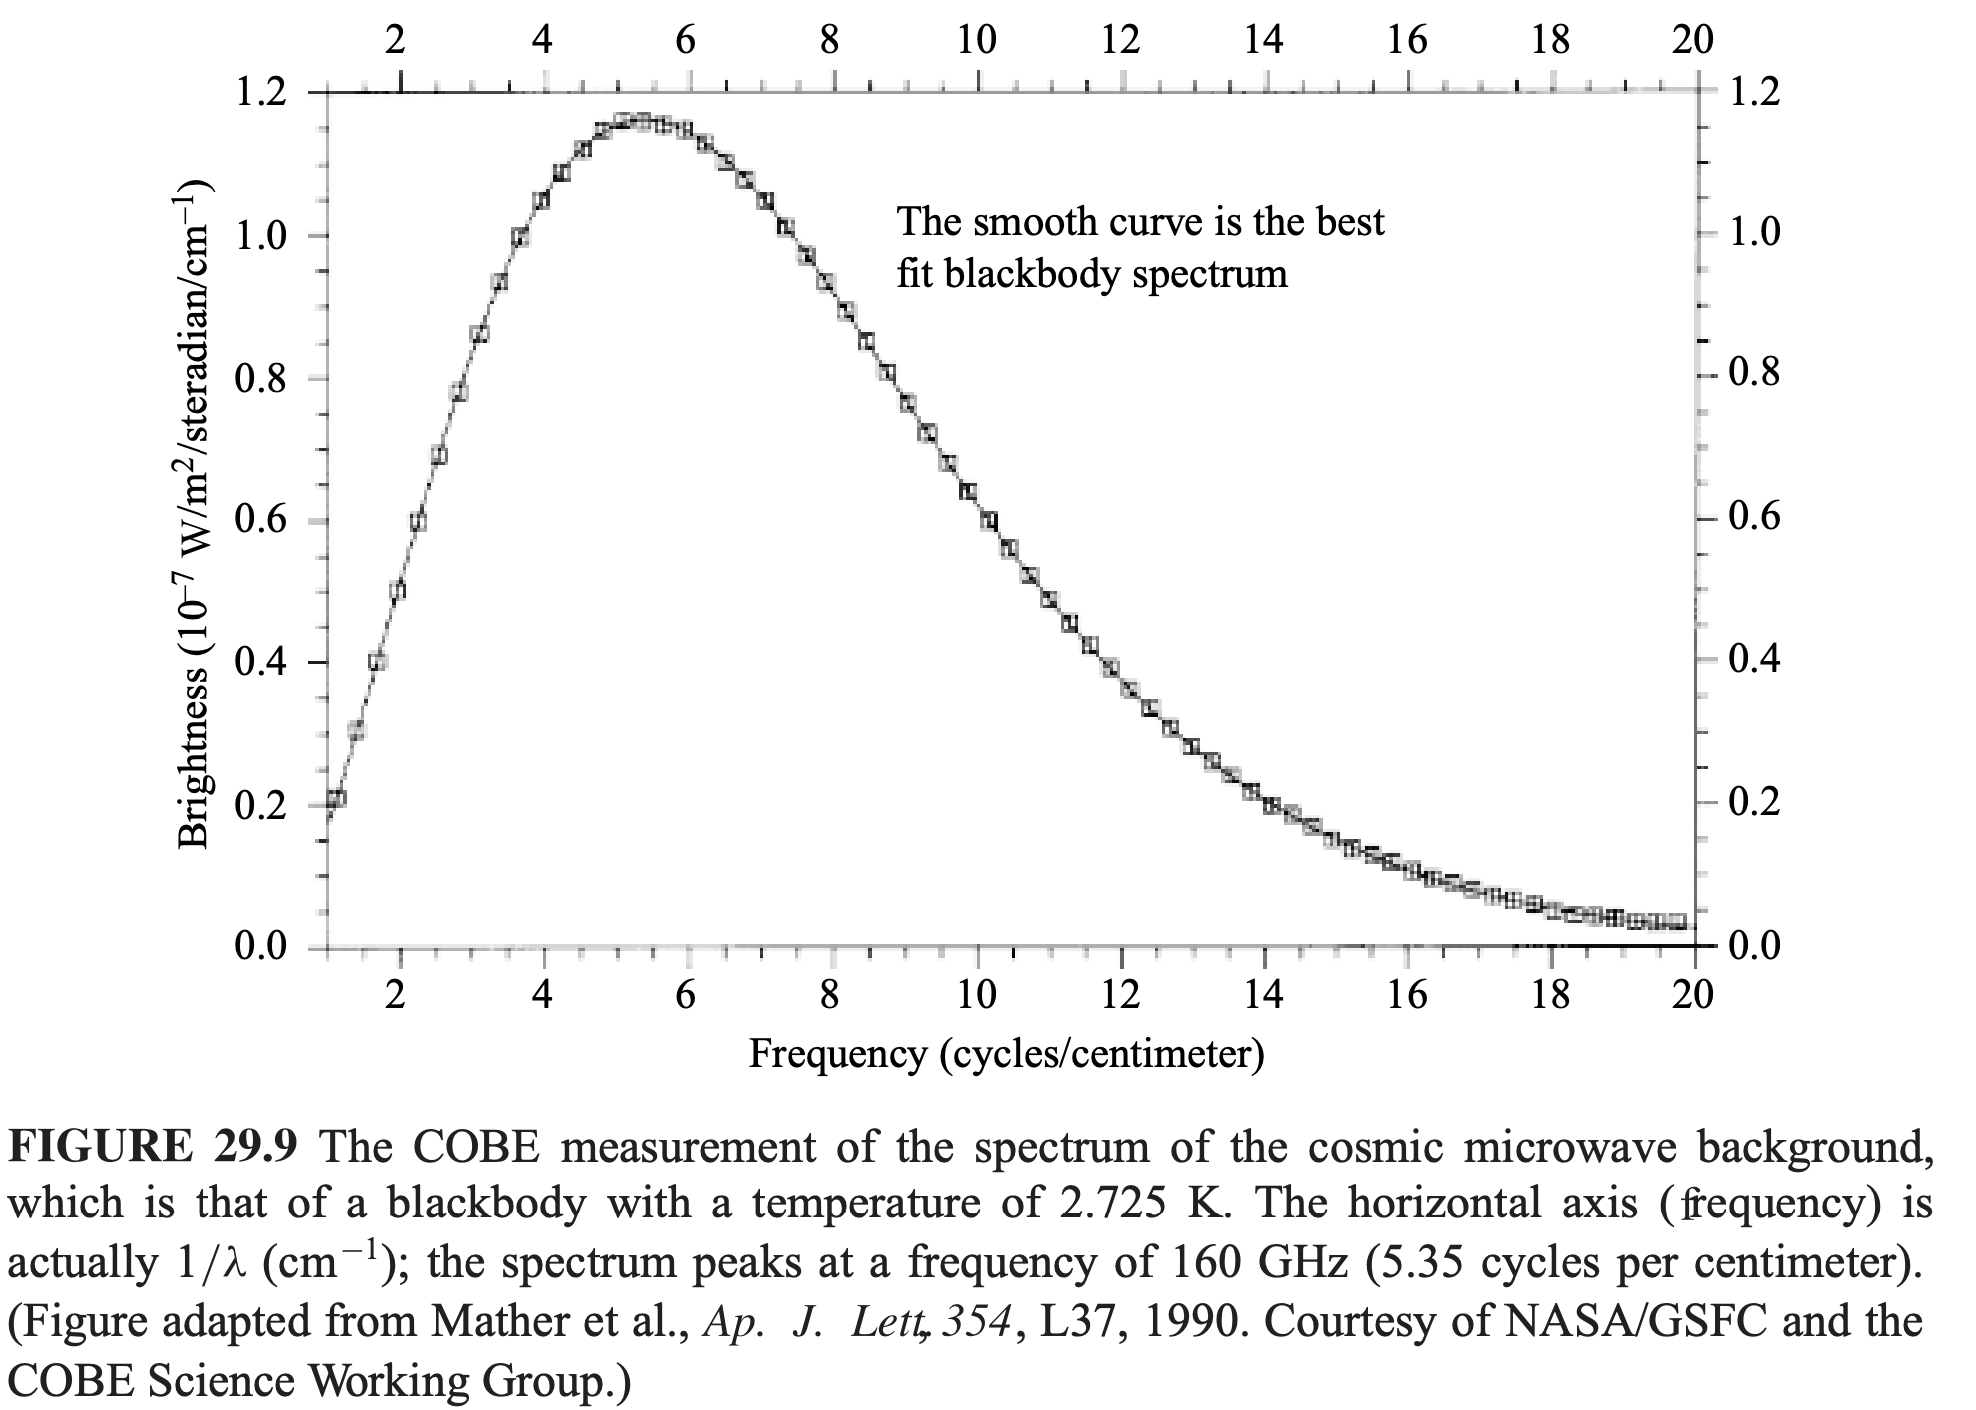
\includegraphics[width = \textwidth]{images/cobe_spec.png}
          \end{center}
          \begin{itemize}
              \item $[T_0]_{\text{WMAP}} = 2.725 \pm 0.002\ K$
              \item $T(z) = T_0 (1 + z)$
          \end{itemize}
    \item Origin
          \begin{itemize}
              \item Early universe was opaque, hot, dense
              \item Recombination: as it expanded, temperature cooled enough for electrons to combine with photons to form hydrogen and helium
              \item Decoupling/surface of last scattering: photons could stream freely for the first time
                    Universe was 380,000 years old
          \end{itemize}
\end{itemize}
\subsection{Big Bang Nucleosynthesis}
\begin{itemize}
    \item Baryonic mass: 74\% Hydrogen, 24\% Helium, 2\% heavier elements
    \item Amount of heavy elements increases with time (more in galaxies with lots of stars/supernova), amount of light elements stars constant with time
    \item For 17 min, Hydrogen and Helium and the other light elements were created via fusion
    \item Boltzmann equation (C\&O 8.6) gives the equilibrium ration of the number density of neutrons, $n_n$, to the number density of protons, $n_p$, as
          \begin{equation*}
              \frac{n_n}{n_p} = \exp\left[ - (m_n - m_p) c^2 / k T \right]
          \end{equation*}
          \begin{itemize}
              \item Going back in time, $n_n / n_p \to 1$
              \item As the universe expands, $n_n / n_p$ decreases as $T$ decreases
          \end{itemize}
    \item Timeline
          \begin{itemize}
              \item $t \sim 10^{-4}$ s and $T \sim 10_{12}$ K: loose particles, universe consisted of protons, neutrons, photons, electrons, positrons, electron and muon neutrons (and their antiparticles). $n_n / n_p = 0.985$
              \item $t \sim 0.01$ s and $T \sim 10^{10}$ K: no long in equilibrium, neutrinos decay into protons. $n_n / n_p$ = 0.223 (freeze-out)
              \item $t \sim 2.9$ min and $T \sim 10^9$ K: hydrogen and helium can form. $n_n / n_p = 0.176$
              \item $t \sim 3 - 20$ min: lighter elements (H, He, Be, Li) fuse (still hot enough, after this it was too cool to fuse)
          \end{itemize}
\end{itemize}
\subsection{Evolution of the Universe}
\begin{itemize}
    \item Friedmann equation: description of the dynamic evolution for the universe (isotropic, homogeneous)
          \begin{equation*}
              \left[  \left( \frac{1}{R} \frac{dR}{dt} \right)^2 - \frac{8}{3} \pi G \rho \right] R^2 = - k c^2 \tag{C\&O 29.107}
          \end{equation*}
    \item With cosmological Constant $\Lambda$, originally to force a static universe
          \begin{equation*}
              \left[  \left( \frac{1}{R} \frac{dR}{dt} \right)^2 - \frac{8}{3} \pi G \rho - \frac{1}{3} \Lambda c^2 \right] R^2 = - k c^2 \tag{C\&O 29.108}
          \end{equation*}
    \item Equivalent mass density of dark energy:
          \begin{equation*}
              \rho_Lambda \equiv \frac{\Lambda c^2}{8 \pi G} = \text{constant} = \rho_{\Lambda, 0} \tag{C\&O 29.113}
          \end{equation*}
          and corresponding Friedmann equation
          \begin{equation*}
              \left[  \left( \frac{1}{R} \frac{dR}{dt} \right)^2 - \frac{8}{3} \pi G (\rho_m + \rho_{rel} + \rho_\Lambda) \right] R^2 = - k c^2 \tag{C\&O 29.114}
          \end{equation*}
    \item Dark matter energy density parameter:
          \begin{equation*}
              \Omega_\Lambda = \frac{\rho_\Lambda}{\rho_c} = \frac{\Lambda c^2}{3 H^2} \tag{C\&O 29.118}
          \end{equation*}
    \item Total density parameter:
          \begin{equation*}
              \Omega \equiv \Omega_m + \Omega_{rel} + \Omega_\Lambda
          \end{equation*}
          where
          \begin{center}
              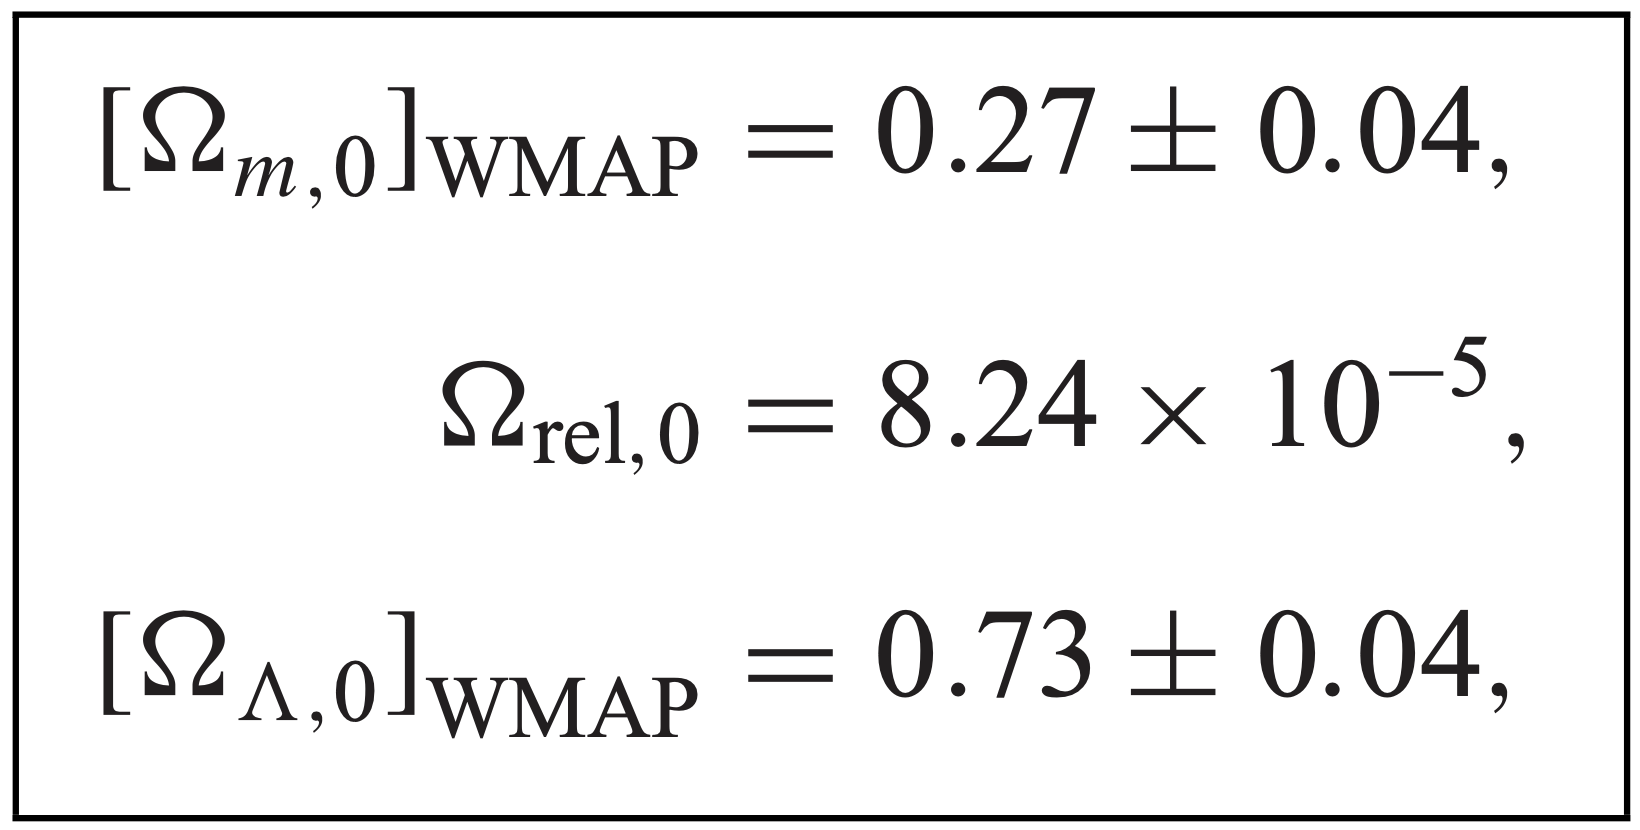
\includegraphics[height = 0.15 \textwidth]{images/total_density.png}
          \end{center}
    \item Adding these results from the Wilkinson Microwave Anisotropy Probe reveals that $$\Omega_0 = \Omega_{m,0} + \Omega_{rel,0} + \Omega-{\Lambda,0} = 1.$$ that is, the universe is flat ($z = 0$), and dark energy now dominates the expansion of the universe.
\end{itemize}
\subsubsection{Acceleration of the Expansion}
\begin{center}
    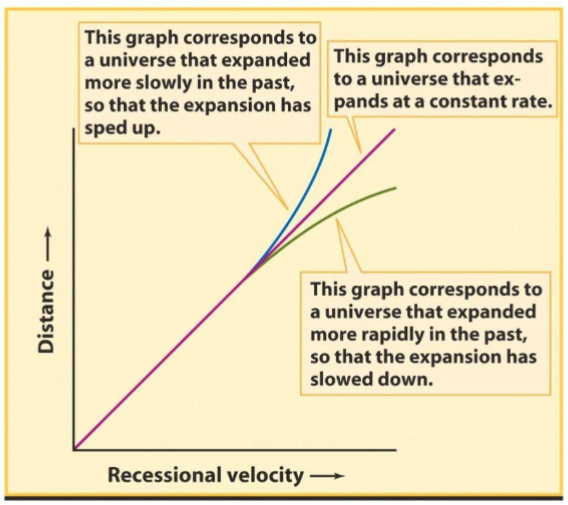
\includegraphics[height = 0.4 \textwidth]{images/accel_exp.png}
\end{center}
\begin{itemize}
    \item Universe is accelerating in its expansion
    \item Expansion was decelerating until $z=0.76$ but it has been accelerating ever since
    \item Source of acceleration is dark energy
    \item Deceleration parameter $q(t)$: a useful dimensionless quantity that describes the acceleration of the universal expansion
          \begin{equation*}
              q(t) \equiv - \frac{R(t) [d^2 R (t)/dt^2]}{[dR(t)/dt]^2} \tag{C\&O 29.54}
          \end{equation*}
          which can also be written as
          \begin{equation*}
              q(t) = \frac{1}{2} \sum_i (1 + 3w_i) \Omega_i (t) \tag{C\&O 29.123}
          \end{equation*}
          where $w$ is the coefficient from the equation of state $P_i = w_i \rho_i c^2$ and the ``$i$'' subscript identifies one of the components of the universe. Using $w_m = 0$, $w_{rel} = 1/3$, and $w_\Lambda = -1$, we obtain
          \begin{equation*}
              q(t) = \frac{1}{2} \Omega_m (t) + \Omega_{rel} (t) - \Omega_\Lambda (t) \overset{\text{WMAP}}{=} -0.60 \tag{C\&O 29.124}
          \end{equation*}
          where the minus sign indicates that the expansion of the universe is now accelerating ($d^2R/dt^2 >0$)!
\end{itemize}
\subsubsection{Dominant Components of the Universe}
\begin{center}
    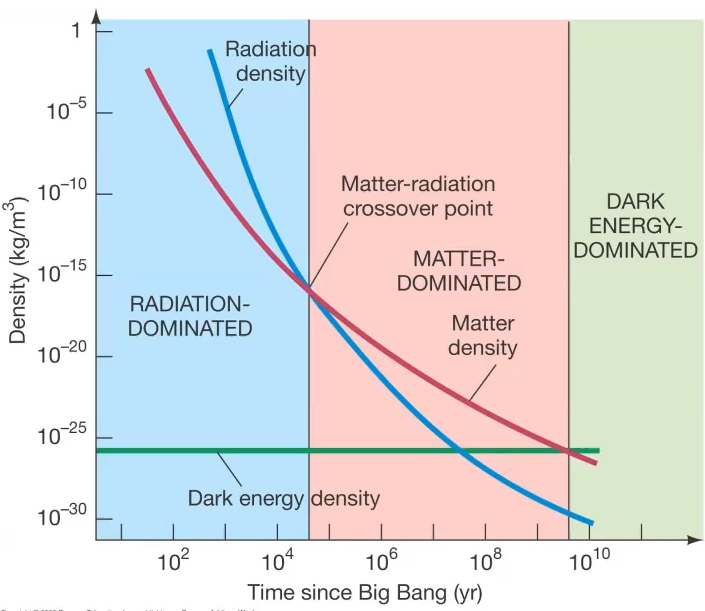
\includegraphics[height = 0.4\textwidth]{images/components.png}
\end{center}
\subsection{Distances (Observational Cosmology)}

\backmatter
\chapter{Topic-Lecture Index}
\begin{table}[H]
    \centering
    \begin{tabular}{|ll|}
        \hline
        \multicolumn{1}{|c}{Topic}      & Lecture \\ \hline \hline
        Welcome to ASTR 3830            & 1       \\ \hline
        Dark Matter                     & 2       \\ \hline
        Galactic Center                 & 3       \\ \hline
        Galaxy Morphologies             & 4       \\ \hline
        Surface Brightness              & 5       \\ \hline
        Spiral Galaxies                 & 6       \\ \hline
        Elliptical Galaxies             & 7       \\ \hline
        Luminosity Function of Galaxies & 8       \\ \hline
        Galactic Evolution              & 9       \\ \hline
        Galactic Evolution              & 10      \\ \hline
        Extragalactic Distance Scale    & 11      \\ \hline
        Extragalactic Distance Scale    & 12      \\ \hline
        Galaxy Clusters                 & 13      \\ \hline
        Galaxy Clusters                 & 14      \\ \hline
        Active Galaxies                 & 15      \\ \hline
        Active Galaxies                 & 16      \\ \hline
        Active Galaxies                 & 17      \\ \hline
        Gravitational Lensing           & 18      \\ \hline
        Cosmology                       & 19      \\ \hline
        Cosmology                       & 20      \\ \hline
        Cosmology                       & 21      \\ \hline
        Cosmology                       & 22      \\ \hline
        Cosmology                       & 23      \\ \hline
        Cosmology                       & 24      \\ \hline
        Cosmology                       & 25      \\ \hline
        Cosmology                       & 26      \\ \hline
    \end{tabular}
\end{table}

\chapter{Potentially Useful Equations}
\begin{itemize}
    \item Integrated Star Count:
          \begin{equation*}
              n(S, \Omega, r) = \int_{- \infty}^\infty n_M (M, S, \Omega, r)\ dM \tag{C\&O 24.2}
          \end{equation*}
          where $n_M (M, S, \Omega, r)$ is the number density of of stars with absolute magnitudes between $M$ and $M+dM$ and attribute $S$ that lie within a solid angle $\Omega$ in a specific direction at a distance $r$ from the observer ($S$ could be composition or the Morgan-Keenan spectral class, for example).
    \item Integrated star count written in terms of limiting distance, $d$:
          \begin{equation*}
              N_M (M, S, \Omega, d)\ dM = \left[ \int_0^d n_M (M, S, \Omega, r) \Omega r^2\ dr \right]\ dM \tag{C\&O 24.3}
          \end{equation*}
    \item Differential Star Count:
          \begin{equation*}
              A_M (M, S, \Omega, m)\ dM\ dm \equiv \frac{d\bar{N}_M (M, S, \Omega, m)}{dm} dM\ dm \tag{C\&O 24.4}
          \end{equation*}
          where $A_M$ is the number of stars with an absolute magnitude between $M$ and $M+dM$ that are found within a solid angle $\Omega$ and have apparent magnitudes in the range between $m$ and $m+dm$.
    \item In the special case where we assume no interstellar extinction ($A=0$) and infinite universe of uniform stellar density (i.e. $n_M(M, S, \Omega, r) = n_M(M, S) = $ constant),
          \begin{align*}
              \bar{N}_M (M, S, \Omega, m) & = \frac{\Omega}{3} n_M (M, S) 10^{3 (m - M + 5)/5}                        \\
                                          & = \frac{\Omega}{3} n_M (M, S) \exp\left( \ln 10^{3 (m - M + 5)/5} \right) \\
                                          & = \frac{\Omega}{3} n_M (M, S) e^{[3 (m - M + 5)/5]\ln 10}
          \end{align*}
    \item In special case where we assume no interstellar extinction ($A=0$) and infinite universe of uniform stellar density (i.e. $n_M(M, S, \Omega, r) = n_M(M, S) = $ constant),
          \begin{align*}
              A_M (M, S, \Omega, m) & = \frac{d\bar{N}_m (M, S, \Omega, m)}{dm}                       \\
                                    & = \frac{\ln 10}{5} \Omega n_m (M, S) 10^{3(m - M +5)/5}         \\
                                    & = \frac{3 \ln 10}{5} \bar{N}_M(M, S, \Omega, r) \tag{C\&O 24.5}
          \end{align*}
    \item Interstellar Extinction:
          \begin{equation*}
              m_\lambda = M_\lambda + 5 \log_{10} d - 5 + A_\lambda \tag{C\&O 12.1}
          \end{equation*}
          where $d$ is the distance in pc and $A_\lambda > 0$ represents the number of magnitudes of interstellar extinction present along the line of sight. We also use two other forms of this equation:
          \begin{align*}
              d         & = 10^{(m_\lambda - M_\lambda - A_\lambda + 5)/5}            \\
              A_\lambda & = m_\lambda - M_\lambda + 5 - 5 \log_{10} d \tag{C\&O 24.1}
          \end{align*}
    \item Perigalacticon (closest approach):
          \begin{equation*}
              r \equiv \frac{a (1 - \epsilon^2)}{1 + \epsilon \cos \theta}
          \end{equation*}
          where the ellipticity
          \begin{equation*}
              \epsilon = 1 - \beta/\alpha \tag{C\&O 25.1}
          \end{equation*}
          and $\alpha$ is the apparent semi-major axis and $\beta$ is the apparent semi-minor axis.
    \item NFW density profile
          \begin{equation*}
              \rho_{NFW} (r) = \frac{\rho_0}{(r/a)(1+r/a)^2} \tag{C\&O 24.52}
          \end{equation*}
          where $rho_0$ and $a$ are choices.
    \item Mass conservation equation and interior mass integral:
          \begin{equation*}
              \frac{dM_r}{dr} = 4 \pi r^2 \rho \implies M_r = \int_0^r 4 \pi r^2 \rho dr \tag{C\&O 10.7}
          \end{equation*}
    \item Virial theorem: for a system that has reached an equilibrium or steady-state configuration,
          \begin{equation*}
              -2 \langle 2 \rangle = \langle U \rangle \tag{C\&O 2.46}
          \end{equation*}
          The theorem may also be expressed in terms of the total energy of the system by using the relation $\langle E \rangle = \langle K \rangle + \langle U \rangle$:
          \begin{equation*}
              \langle E \rangle = \frac{1}{2} \langle U \rangle
          \end{equation*}
    \item Flux is related to an object's luminosity by
          \begin{equation*}
              F = \frac{L}{4 \pi r^2} \tag{C\&O 3.2}
          \end{equation*}
          We can also define the flux ratio of two stars:
          \begin{equation*}
              \frac{F_2}{F_1} = 100^{(m_1 - m_2)/5}
          \end{equation*}
\end{itemize}
\end{document}